\documentclass[12pt,a4paper,titlepage,headinclude,bibtotoc]{scrartcl}
%---- Allgemeine Layout Einstellungen ------------------------------------------

% Für Kopf und Fußzeilen, siehe auch KOMA-Skript Doku
\usepackage[komastyle]{scrpage2}
\pagestyle{plain}
\setheadsepline{0.5pt}[\color{black}]
\automark[section]{chapter}


%Einstellungen für Figuren- und Tabellenbeschriftungen
\setkomafont{captionlabel}{\sffamily\bfseries}
\setcapindent{0em}


%---- Weitere Pakete -----------------------------------------------------------
% Die Pakete sind alle in der TeX Live Distribution enthalten. Wichtige Adressen
% www.ctan.org, www.dante.de

% Sprachunterstützung
\usepackage[ngerman]{babel}

% Benutzung von Umlauten direkt im Text
% entweder "latin1" oder "utf8"
\usepackage[utf8]{inputenc}

% Pakete mit Mathesymbolen und zur Beseitigung von Schwächen der Mathe-Umgebung
\usepackage{latexsym,exscale,stmaryrd,amssymb,amsmath}


\usepackage[nointegrals]{wasysym}
\usepackage{eurosym}

% Anderes Literaturverzeichnisformat
%\usepackage[square,sort&compress]{natbib}
%\usepackage{hyperref}
\usepackage{url}
% Für Farbe
\usepackage{color}
\usepackage{graphicx}
\usepackage{wrapfig}
\usepackage{subfigure}

% Caption neben Abbildung
\usepackage{sidecap}


% Befehl für "Entspricht"-Zeichen
\newcommand{\corresponds}{\ensuremath{\mathrel{\widehat{=}}}}
% Befehl für Errorfunction
\newcommand{\erf}[1]{\text{ erf}\ensuremath{\left( #1 \right)}}


%Fußnoten zwingend auf diese Seite setzen
\interfootnotelinepenalty=1000

%Für chemische Formeln (von www.dante.de)
%% Anpassung an LaTeX(2e) von Bernd Raichle
\makeatletter
\DeclareRobustCommand{\chemical}[1]{%
  {\(\m@th
   \edef\resetfontdimens{\noexpand\)%
       \fontdimen16\textfont2=\the\fontdimen16\textfont2
       \fontdimen17\textfont2=\the\fontdimen17\textfont2\relax}%
   \fontdimen16\textfont2=2.7pt \fontdimen17\textfont2=2.7pt
   \mathrm{#1}%
   \resetfontdimens}}
\makeatother
\usepackage{textcomp}
\usepackage{upgreek}
%\begin{document}
%$\upmu$
%\end{document}
%Honecker-Kasten mit $$\shadowbox{$xxxx$}$$
\usepackage{fancybox}

%SI-Package
\usepackage{siunitx}

%keine Einrückung, wenn Latex doppelte Leerzeile
\parindent0pt

%Bibliography \bibliography{literatur} und \cite{gerthsen}
%\usepackage{cite}
\usepackage{babelbib}
\selectbiblanguage{ngerman}

\usepackage{siunitx}
%\begin{document}
 % \SI{1.55}{\micro\metre}
\sisetup{math-micro=\text{µ},text-micro=µ}
\usepackage{amsmath}

\usepackage{siunitx}
%\begin{document}
 % \SI{1.55}{\micro\metre}
\sisetup{math-micro=\text{µ},text-micro=µ}
\usepackage{amsmath}
\usepackage[verbose]{placeins}
\usepackage{setspace}
\usepackage{threeparttable}
\usepackage[verbose]{placeins}
\usepackage[justification=centering]{caption}


\begin{document}

\begin{titlepage}
\centering
\textsc{\Large Physikalisch- Chemisches Grundpraktikum\\[1.5ex] Universität Göttingen}

\vspace*{0.5cm}

\rule{\textwidth}{1pt}\\[0.5cm]
{\huge \bfseries
  Versuch 6: \\[1.5ex]
  Verbrennungswärme von Naphthalin}\\[0.5cm]
\rule{\textwidth}{1pt}

\vspace*{0.5cm}

\begin{Large}
\begin{tabular}{ll}
Durchführende: &  Isaac Maksso, Julia Stachowiak\\
Assistent: & Jannis Neugebohren\\
Versuchsdatum: & 08.12.2016\\
Datum der ersten Abgabe: & 15.12.2016\\
Datum der zweiten Abgabe: & 22.12.2016\\
\end{tabular}
\end{Large}

\vspace*{0.5cm}

\vspace{1.3cm} 
\end{titlepage}


\tableofcontents %=Inhaltsverzeichnis
\newpage
 
 \section{Experimentelles}

\subsection{Versuchsaufbau}
\begin{figure} [ht!]
\begin{center}
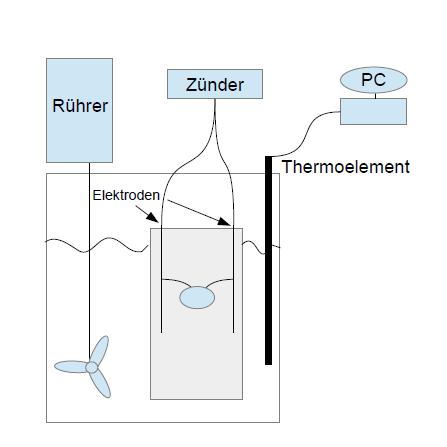
\includegraphics[scale=0.9]{Versuchsaufbau.png} \end{center}
\caption{Versuchsaufbau: Die aus der gepressten Tablette führenden Enden des Nickeldrahtes sind an den Elektroden des Gestells befestigt; dieses befindet sich in einer fest zugeschraubten Bombe. Der Pt100-Temperaturmesskopf\,(elektronische Weitergabe der Daten an den Computer), sowie der Rührer befinden sich im Wasser. Die Apparatur ist vollständig mit Flüssigkeit bedeckt und mit einem leichten Metalldeckel abgedeckt.}
\end{figure}

\subsection{Durchführung}
Die Verbrennungswärme von Naphthalin sollte mittels eines Kalorimeters mit Berthelot-Mahlerscher Bombe ermittelt werden.\\
Zur Kalibrierung des Thermoelements wurden ca. 0,6 g mit einem vorher gedrehten und genau gewogenen Nickeldraht in eine Tablette gepresst. An einer Stelle wurde vorher eine Spur des doppelt gewickelten Drahtes durchtrennt und so gelegt, dass sich diese Zündungsstelle innerhalb der Tablette befand. Die Tablette wurde am Nickeldraht an zwei Elektroden befestigt und die Bombe angeschraubt. Anschließend wurde diese mit 25 atm O$_2$ befüllt und in das Wasserbad gestellt.  Die Temperaturmessung erfolgte über einen Pt100-\,Temperaturmesskopf (Verstärkung mit einem Pt100-Vorverstärker um 20\,mV$\cdot$K$^{-1}$). Nach ca. 3 Minuten Vorperiode wurde die Probe gezündet und ca. 5 Minuten lang weitergemessen\,(Nachperiode).
Die Temperaturaufzeichung erfolgte mittels LabView.\\
Der Vorgang wurde mit Benzoesäure\,(zur Ermittlung der Wärmekapazität des Kalorimeters) und Naphthalin je drei mal durchgeführt.\\ 

\section{Auswertung}
Für die Verbrennung von Naphthalin (\ref{Naphthalin}) und Benzoesäure (\ref{Benzoesaeure}) ergeben sich folgende Reaktionsgleichungen:\\

\begin{equation}\label{Benzoesaeure}
\mathrm{C_6}\mathrm{H}_5\mathrm{COOH}_\mathrm{(s)} + 7,5\,{\mathrm{O}_2}_\mathrm{(g)} \rightarrow 7\,{\mathrm{CO}_2}_\mathrm{(g)} +3\,\mathrm{H}_2\mathrm{O}_\mathrm{(l)}
\end{equation}

\begin{equation}\label{Naphthalin}
{\mathrm{C}_{10}\mathrm{H}_8}_\mathrm{(s)} + 12\,{\mathrm{O}_2}_\mathrm{(g)} \rightarrow 10\,{\mathrm{CO}_2}_\mathrm{(g)} + 4\,\mathrm{H}_2\mathrm{O}_\mathrm{(l)}
\end{equation}

Nach dem Satz von Hess kann die Reaktionsenthalpie aus der Differenz der Standardbildungsenthalpien $\Delta H_\mathrm{f}^0$ zwischen Produkten und Edukten berechnet werden:\\

\begin{equation} \label{GleichungHess}
\Delta H_\mathrm{C} = \sum_i \nu_i\Delta H_{\mathrm{f},i}\mathrm{(Produkte)} - \sum_i \nu_i\Delta H_{\mathrm{f},i}\mathrm{(Edukte)}
\end{equation}

Die Literaturwerte für die molaren Standardbildungsenthalpien\,$\Delta H_{\mathrm{f,m}}$ und die nach Gleichung\,(\ref{GleichungHess}) berechneten Verbrennungsenthalpien $\Delta H_\mathrm{C,m}$ für Benzoesäure und Naphthalin sind in  Tabelle
(1)
%(\ref{tab:LiteraturwerteBildungsenthalpien})
aufgelistet.\\

\begin{center}
\begin{table} [ht!] \label{tab:LiteraturwerteBildungsenthalpien}
\caption{Molare Standardbildungsenthalpien sowie Verbrennungsenthalpien für Benzoesäure und Naphthalin.}
\centering
\begin{tabular}{c|c|c} 
  & $\Delta H_{\mathrm{f,m}}$ [kJ$\cdot$mol$^{-1}$] &$\Delta H_\mathrm{C,m}$[kJ$\cdot$mol$^{-1}$]\\ 
 \hline 
 $\mathrm{C}_6\mathrm{H}_5\mathrm{COOH}_\mathrm{(s)}$ & -384,8$^2$&-3227 \\ 
 \hline 
 ${\mathrm{C}_{10}\mathrm{H}_8}_\mathrm{(s)}$ & 78,53$^3$ &-5157\\
 \hline 
 ${\mathrm{O}_2}_\mathrm{(g)}$ & 0$^1$ \\ 
 \hline 
 ${\mathrm{CO}_2}_\mathrm{(g)}$ & -393,51$^1$ \\ 
 \hline 
 $\mathrm{H}_2\mathrm{O}_\mathrm{(l)}$ & –285,830$^1$ \\ 
 \end{tabular}  
\end{table}
\end{center}
\FloatBarrier


Die aus den Auftragungen ermittelten Temperaturdifferenzen sind in Tabelle\,(2)
%(\ref{TabDeltaT})
 dargestellt. \\

\begin{center}
\begin{table} [ht!] \label{TabDeltaT}
\centering
\caption{Aus den Auftragungen ermittelte Temperaturdifferenzen.}
\begin{tabular}{c|c|c|c|c|c|c}
&\multicolumn{3}{c|}{Benzoesäure} & \multicolumn{3}{c}{Naphthalin}\\ 
Messung& 1&2&3&1&2&3\\
\hline 
$\Delta T$ /K & 1,21 & 1,17 & 1,15 & 2,31 & 1,88 & 2,05 \\ 
$m$ /g&0,6460&0,6044&0,6208&0,8229&0,6166&0,7072\\
$n$ /mmol& 5,288&4,949&5,084&6,420&4,811&5,518\\
\end{tabular} 
\end{table}
\end{center}
\FloatBarrier

\subsection{Bestimmung der Wärmekapazität des Kalorimeters und der Änderung der inneren Energie}
Die Wärmekapazität bei konstantem Volumen ist folgendermaßen definiert:\\

\begin{equation}
C_v = \left(\frac{\delta Q}{\partial T}\right)_v = \left(\frac{\partial U}{\partial T}\right)_v
\end{equation}

Integration liefert einen Differenzenquotienten. Die zugeführte Wärmemenge $\delta Q$ muss mit $(-1)$ multipliziert werden, da es sich um die vom Kalorimeter aufgenommene Wärmemenge handelt. Da mit der molaren Änderung der inneren Energie $\Delta U_\mathrm{C,m}$ gerechnet wird, ergibt sich die molare Wärmekapazität. Um den absoluten Wert zu erhalten wird diese daher mit der Stoffmenge multipliziert:\\

\begin{equation}\label{Waermekapazitaet}
C_v= - \frac{\Delta U_\mathrm{C,m}}{\Delta T} \cdot n
\end{equation}

\newpage
Das totale Differential der inneren Energie lautet folgendermaßen:\\

\begin{equation}
\mathrm{d}U= T\mathrm{d}S - p\mathrm{d}V
\end{equation} 

Bei konstantem Volumen fällt der letzte Term weg und folgender Zusammenhang mit der Enthalpie besteht:\\

\begin{equation} 
\mathrm{d}H|_v= T\mathrm{d}S + V\mathrm{d}p = \mathrm{d}U + V\mathrm{d}p = \mathrm{d}U +\mathrm{R}T_0\sum_i \nu_{i,gas}
\end{equation}

Der letzte Term beschreibt dabei die Änderung der Stoffmenge ($\mathrm{d}n= \sum_i \nu_{i,gas}$). Integration liefert:\\


\begin{equation} \label{Gl61}
\Delta H_\mathrm{C}= \Delta U_\mathrm{C} +V\Delta p= \Delta U_\mathrm{C} +\mathrm{R}T_0\sum_i \nu_{i,gas}
\end{equation}

Für Benzoesäure kann die Wärmekapazität nach Gleichung (\ref{Waermekapazitaet}) und die Änderung der inneren Energie nach Gleichung (\ref{Gl61}) bestimmt werden. $T_0$ beschreibt dabei die Anfangstemperatur\,der Messung. Nach der Reaktionsgleichung für die Verbrennung von Benzoesäure ergibt sich $\sum \nu_{i,\mathrm{gas}}= -0,5$. Die Ergebnisse sind in Tabelle (3) dargestellt.\\

\begin{table} \centering
\label{ErgebnisseBenz}\caption{Die molare Wärmekapazität und Änderung der inneren Energie für Benzoesäure.}
\begin{tabular}{c|c|c|c}
Messung& 1&2&3\\
\hline 
$T_0$ /K&294,584&295,909&301,017\\
$\Delta U_\mathrm{C,m}$ /kJ$\cdot \mathrm{mol}^{-1}$&
-3225,8&-3225,8&-3225,7\\
$C_{v}$ /kJ$\cdot \mathrm{K}^{-1}$&14,102&13,645&14,259\\
\end{tabular} 
\end{table}
\FloatBarrier

\subsection{Bestimmung der Verbrennungsenthalpie $\Delta H_\mathrm{C,m}$ von Naphthalin}

Mit der molaren Wärmekapazität des Thermoelements kann die molare Verbrennungswärme $\Delta Q_{\mathrm{C,m}}$von Naphthalin berechnet werden. Diese ist gleich der molaren Änderung der inneren Energie $\Delta U_\mathrm{C,m}$. Da die Wärmekapazität durch die vom Kalorimeter aufgenommene Wärme bestimmt wird und hier mit der bei der Verbrennung frei werdenden Wärme gerechnet wird, muss mit $(-1)$ multpliziert werden.\\

\begin{equation}
\Delta U_\mathrm{C,m}= \Delta Q_\mathrm{C,m}= - \frac{C_{v,\mathrm{m}}\cdot \Delta T}{n}
\end{equation}

Einsetzen in Gleichung (\ref{Gl61}) mit $\sum_i \nu_i$= -2 liefert die Verbrennungsenthalpie $\Delta H_\mathrm{C,m}$. Es wurde mit dem Mittelwert von $C_v$ gerechnet. Die Ergebnisse sind in Tabelle (4)
%(\ref{Endergebnisse})
 zu sehen.\\

\begin{table}[ht!]\centering 
\caption{Molare Verbrennungswärme und Verbrennungsenthalpie für Naphthalin.}  \label{Endergebnisse}
\begin{tabular}{c|c|c|c}
Messung & 1 & 2 & 3 \\ 
\hline 
$T_0$ /K &298,14&300,2&300,9\\
\hline 
$\Delta U_\mathrm{C,m}$ /J$\cdot$mol$^{-1}$ 
&-5037,9&-5471,9&-5202,3\\
\hline 
$\Delta H_\mathrm{C,m}$ /J$\cdot$mol$^{-1}$ 
&-5042,9&-5476,9&-5207,3\\
\end{tabular} 
\end{table}
\FloatBarrier

\subsection{Berechnung der Standardbildungsenthalpie $\Delta H_\mathrm{f,m}$ von Napthalin}

Mit der molaren Verbrennungsenthalpie $\Delta H_\mathrm{C,m}$ von Naphthalin kann nach dem Satz von Hess (Gleichung \ref{GleichungHess}) auf die molare Standardbildungsenthalpie zurückgerechnet werden und so die Genauigkeit der Messung geprüft werden:\\

\begin{equation}
\Delta H_\mathrm{f,m}({\mathrm{C}_{10}\mathrm{H}_8}_\mathrm{(s)}) = -\Delta H_\mathrm{C,m} +7\cdot \Delta H_\mathrm{f,m}({\mathrm{CO}_2}_\mathrm{(g)}) + 3\cdot \Delta H_\mathrm{f,m}({\mathrm{H}_2\mathrm{O}}_\mathrm{(l)}) 
\end{equation}

Folgende Werte ergeben sich:\\

\begin{table}[ht!]\centering  \caption{Nach dem Satz von Hess errechnete Standardbildungsenthalpien für Naphthalin.}
\begin{tabular}{c|c}
Messung & $\Delta H_\mathrm{f,m}^\mathrm{exp.}$ /kJ$\cdot$mol$^{-1}$\\ 
\hline
1 & -35,526\\ 
\hline 
2 & 398,52 \\ 
\hline 
3 & 128,93 \\ 
\end{tabular} 
\end{table}

\subsection{Fehlerrechnung}
Folgende Fehler treten auf:\\
 $\Delta m$= 0,0001 g\\
 $\Delta T_0$= 0,1 K\\
 
Die Fehler der Temperaturdifferenzen ergeben sich aus Grenzgeraden der Auftragungen: $\Delta \Delta T= \frac{\Delta T_\mathrm{max}-\Delta T_\mathrm{min}}{2} $. Aus Gründen der besseren Übersichtlichkeit wurden die Fehlerbalken nicht für jeden Wert eingezeichnet. Die Auftragungen mit den Fehlerbalken sind im Anhang zu finden; die Fehler für $\Delta T$ sind in Tabelle\,(6)
%(\ref{TabDeltaDeltaT})
 dargestellt.\\

\begin{table}[ht!]\centering  \caption{$\Delta \Delta T$ /K für jede Auftragung.} \label{TabDeltaDeltaT}
\begin{tabular}{c|c|c}
Messung & Benzoesäure & Naphthalin \\ 
\hline 
1 & 0,16 & 0,09 \\ 
\hline 
2 & 0,16 & 0,17 \\ 
\hline 
3 & 0,14 & 0,18 \\ 
\end{tabular} 
\end{table}
\FloatBarrier

Die Fehler ergeben sich als Größtfehler:\\

\begin{equation}
\Delta f=\sum_i \left| \left(\frac{\partial f}{\partial x_i}\right)\right| \cdot \Delta x_i
\end{equation}

Die Fehler für $C_{v}$ und $\Delta H_\mathrm{C,m}$  ergeben sich folgendermaßen (mit $\Delta n= \frac{\Delta m}{\mathrm{M}})$:\\

\begin{equation}
\Delta C_{v}= \left|-\left(\frac{-\Delta H_\mathrm{C,m}-0,5 \cdot \mathrm{R}\cdot T_0}{\Delta T^2}\right) \cdot n\right|\cdot \Delta \Delta T + \left|\left(\frac{-0,5 \cdot \mathrm{R}}{\Delta T}\right) \cdot n\right| \cdot \Delta T_0+ \left|\frac{-\Delta H_\mathrm{C,m}-0,5 \cdot \mathrm{R}\cdot T_0}{\Delta T}\right|\cdot \Delta n
\end{equation}

%\begin{equation}
%\Delta \Delta H_\mathrm{f,m}=\Delta \Delta H_\mathrm{C,m}= \left|\frac{1}{\Delta T}\right| \cdot \Delta C_{v}+ \left|-\frac{C_{v}}{\Delta T^2}\right|\cdot \Delta \Delta T+\left|-2\mathrm{R}\right| \cdot \Delta T
%\end{equation}

\begin{equation}
\Delta \Delta H_\mathrm{f,m}=\Delta \Delta H_\mathrm{C,m}=\left|-\frac{\Delta T}{n}\right|\cdot \Delta C_v +\left|-\frac{C_v}{n}\right| \cdot \Delta\Delta T + \left|\frac{C_v \cdot \Delta T}{n^2}\right|\cdot \Delta n +\left|\mathrm{R}\cdot \nu_{i,\mathrm{gas}}\right| \cdot \Delta T_0
\end{equation}

Die Ergebnisse sind in Tabelle\,(\ref{TabBerechneteFehler}) zu sehen.\\


\begin{table}[ht!]\centering  \caption{Fehler $C_v$ und $H_\mathrm{C,m}$.}\label{TabBerechneteFehler}
\begin{tabular}{c|c|c|c} 
 & Messung & $\Delta C_{v}$ /kJ$\cdot$ K$^{-1}$ & $\Delta H_\mathrm{C,m}$ /kJ$\cdot$mol$^{-1}$\\ 
\hline 
Benzoesäure & 1 & 1,9 &  \\ 
\hline 
 & 2 & 1,9 &  \\ 
\hline 
 & 3 & 1,7 &  \\ 
\hline 
Naphthalin & 1 &  & 85$\cdot 10^1$ \\ 
\hline 
 & 2 &  & 12$\cdot 10^2$ \\ 
\hline 
 & 3 & & 11$\cdot 10^2$ \\ 
\end{tabular} 
\end{table}
\FloatBarrier


\section{Fehlerdiskussion}

\begin{table}[ht!]\centering  \caption{Ergebnisse und Literaturwerte.}
\begin{tabular}{c|c|c|c|c|c|c}
 &\multicolumn{3}{c|}{$\Delta H_\mathrm{C,m}$ /kJ$\cdot$mol$^{-1}$}& \multicolumn{3}{c}{$\Delta H_\mathrm{f,m}$ /kJ$\cdot$mol$^{-1}$}\\ 
\hline 
Messung & 1 & 2 & 3 & 1 & 2 & 3 \\
$T_0$ /K&298,14&300,2&300,9&298,14&300,2&300,9\\
Wert &-5040$\pm$850&-5500$\pm$1200&-5200$\pm$1100&-40$\pm$900&400$\pm$1200&100$\pm$1000\\
\hline
Literaturwert&\multicolumn{3}{c|}{-5157$^3$}&\multicolumn{3}{c}{78,53$^3$}\\
\end{tabular} 
\end{table}








Die Abweichung der Werte zu den Literaturwerten ist extrem groß und liegt sehr stark außerhalb der Fehlergrenzen. Die Abweichung aller Werte ist ungefähr gleich groß und erstreckt sich über 2 Zehnerpotenzen, die Streuung verhältnismäßig klein. Dies lässt auf sehr starke systematische Fehler schließen, die im Folgenden diskutiert werden.
Da die Standardbildungsenthalpie mit der Verbrennungsenthalpie berechnet wurde, sind die Abweichungen gleich groß. \\

Die letzte Auftragung von Benzoesäure sowie die letzen beiden Auftragungen von Naphthalin weisen einen sehr untypischen, zackigen Verlauf auf. Dieser kann durch Verunreinigungen, Ausfallen des Rührers oder ein defektes Thermoelement entstanden sein. Die Auswertung dieser Kurven erlaubt nur eine sehr ungenaue Bestimmung der  Temperaturdifferenz. Dennoch weichen die Werte nicht überverhältnismäßig stark von den Temperaturdifferenzen mit geradem Kurvenverlauf ab. Dies deutet auf andere systematische Fehlerquellen hin, die alle Messungen gleichermaßen beeinflusst haben.\\

Auffällig sind die starken Schwankungen in der Anfangsesstemperatur um ca. 5 K (z.B. bei der ersten und letzten Messung von Benzoesäure). Es kann sein, dass das Wasser von der vorigen Messung nicht richtig abgekühlt ist. Allerdings betrug die während des Versuchs gemessene Temperaturdifferenz nur 1-2 K, sodass dies nicht die Hauptursache gewesen sein kann. Wahrscheinlich war das Referenzbad des Thermoelements unstetig. Die somit ungenaue Anfangstemperatur ist damit zusätzlich fehlerbehaftet. Eine zu geringe Temperatur würde eine größere Enthalpie verursachen.\\

Während der Rechnung wird die Wärmekapazität als konstant, d.h. temperaturunabhängig betrachtet und mit der Anfangstemperatur der Messung gerechnet. Tatsächlich wird diese mit steigender Temperatur größer, sodass der Wert der Wärmekapazität systematisch zu klein sein muss. Dies führt ebenfalls zu einem zu geringen Wert von $\Delta U$ und somit auch $\Delta H$.\\

Bei der Berechnung der Verbrennungswärme wurde außerdem die Wärmekapazität des Kalorimeters bei einer leicht anderen Temperatur verwendet. Es wurde nicht der Mittelwert aus den drei Messungen gebildet, sodass möglicherweise mit einem besonders fehlerbehafteten Wert gerechnet wurde und sich diese Ungenauigkeit fortgepflanzt hat.\\

Ob immer eine vollständige Umsetung in die Produkte stattgefunden hat, ist nicht bestimmbar, würde die Messung aber auch stark systematisch verfälschen.\\
Des weiteren liegt kein ideal adiabatisches System vor, sodass während der Messung Wärme entweichen konnte und die gemessene Temperaturerhöhung zu gering ist. Dies hat eine zu groß bestimmte Wärmekapazität des Kalorimeters zur Folge und wiederum eine zu große Änderung der inneren Energie und somit auch Enthalpie.\\

Für die letzte Messung war Naphthalin schwer in der Apparatur zu befestigen, wobei noch nach dem Wiegen ein Massenverlust stattgefunden haben muss. Da der Wert für die 3. Messung jedoch nicht groß abweicht, hatte dieser Fehler wahrscheinlich nur einen kleinen Effekt.\\
 


%gerechnet mit Standardbildungsenthalpien; heißt bei Standardbedingungen 25 Grad die wir aber nicht hatten\\


%Fehlerbestimmung schwierig wenn nur kurze Nachlaufperiode, wie zB. bei Benz2 (schwierig mit den Grenzgeraden)

\newpage
\section{Anhang}
\subsection{Auftragungen der Messungen}
\begin{figure} [h!]
\begin{center}
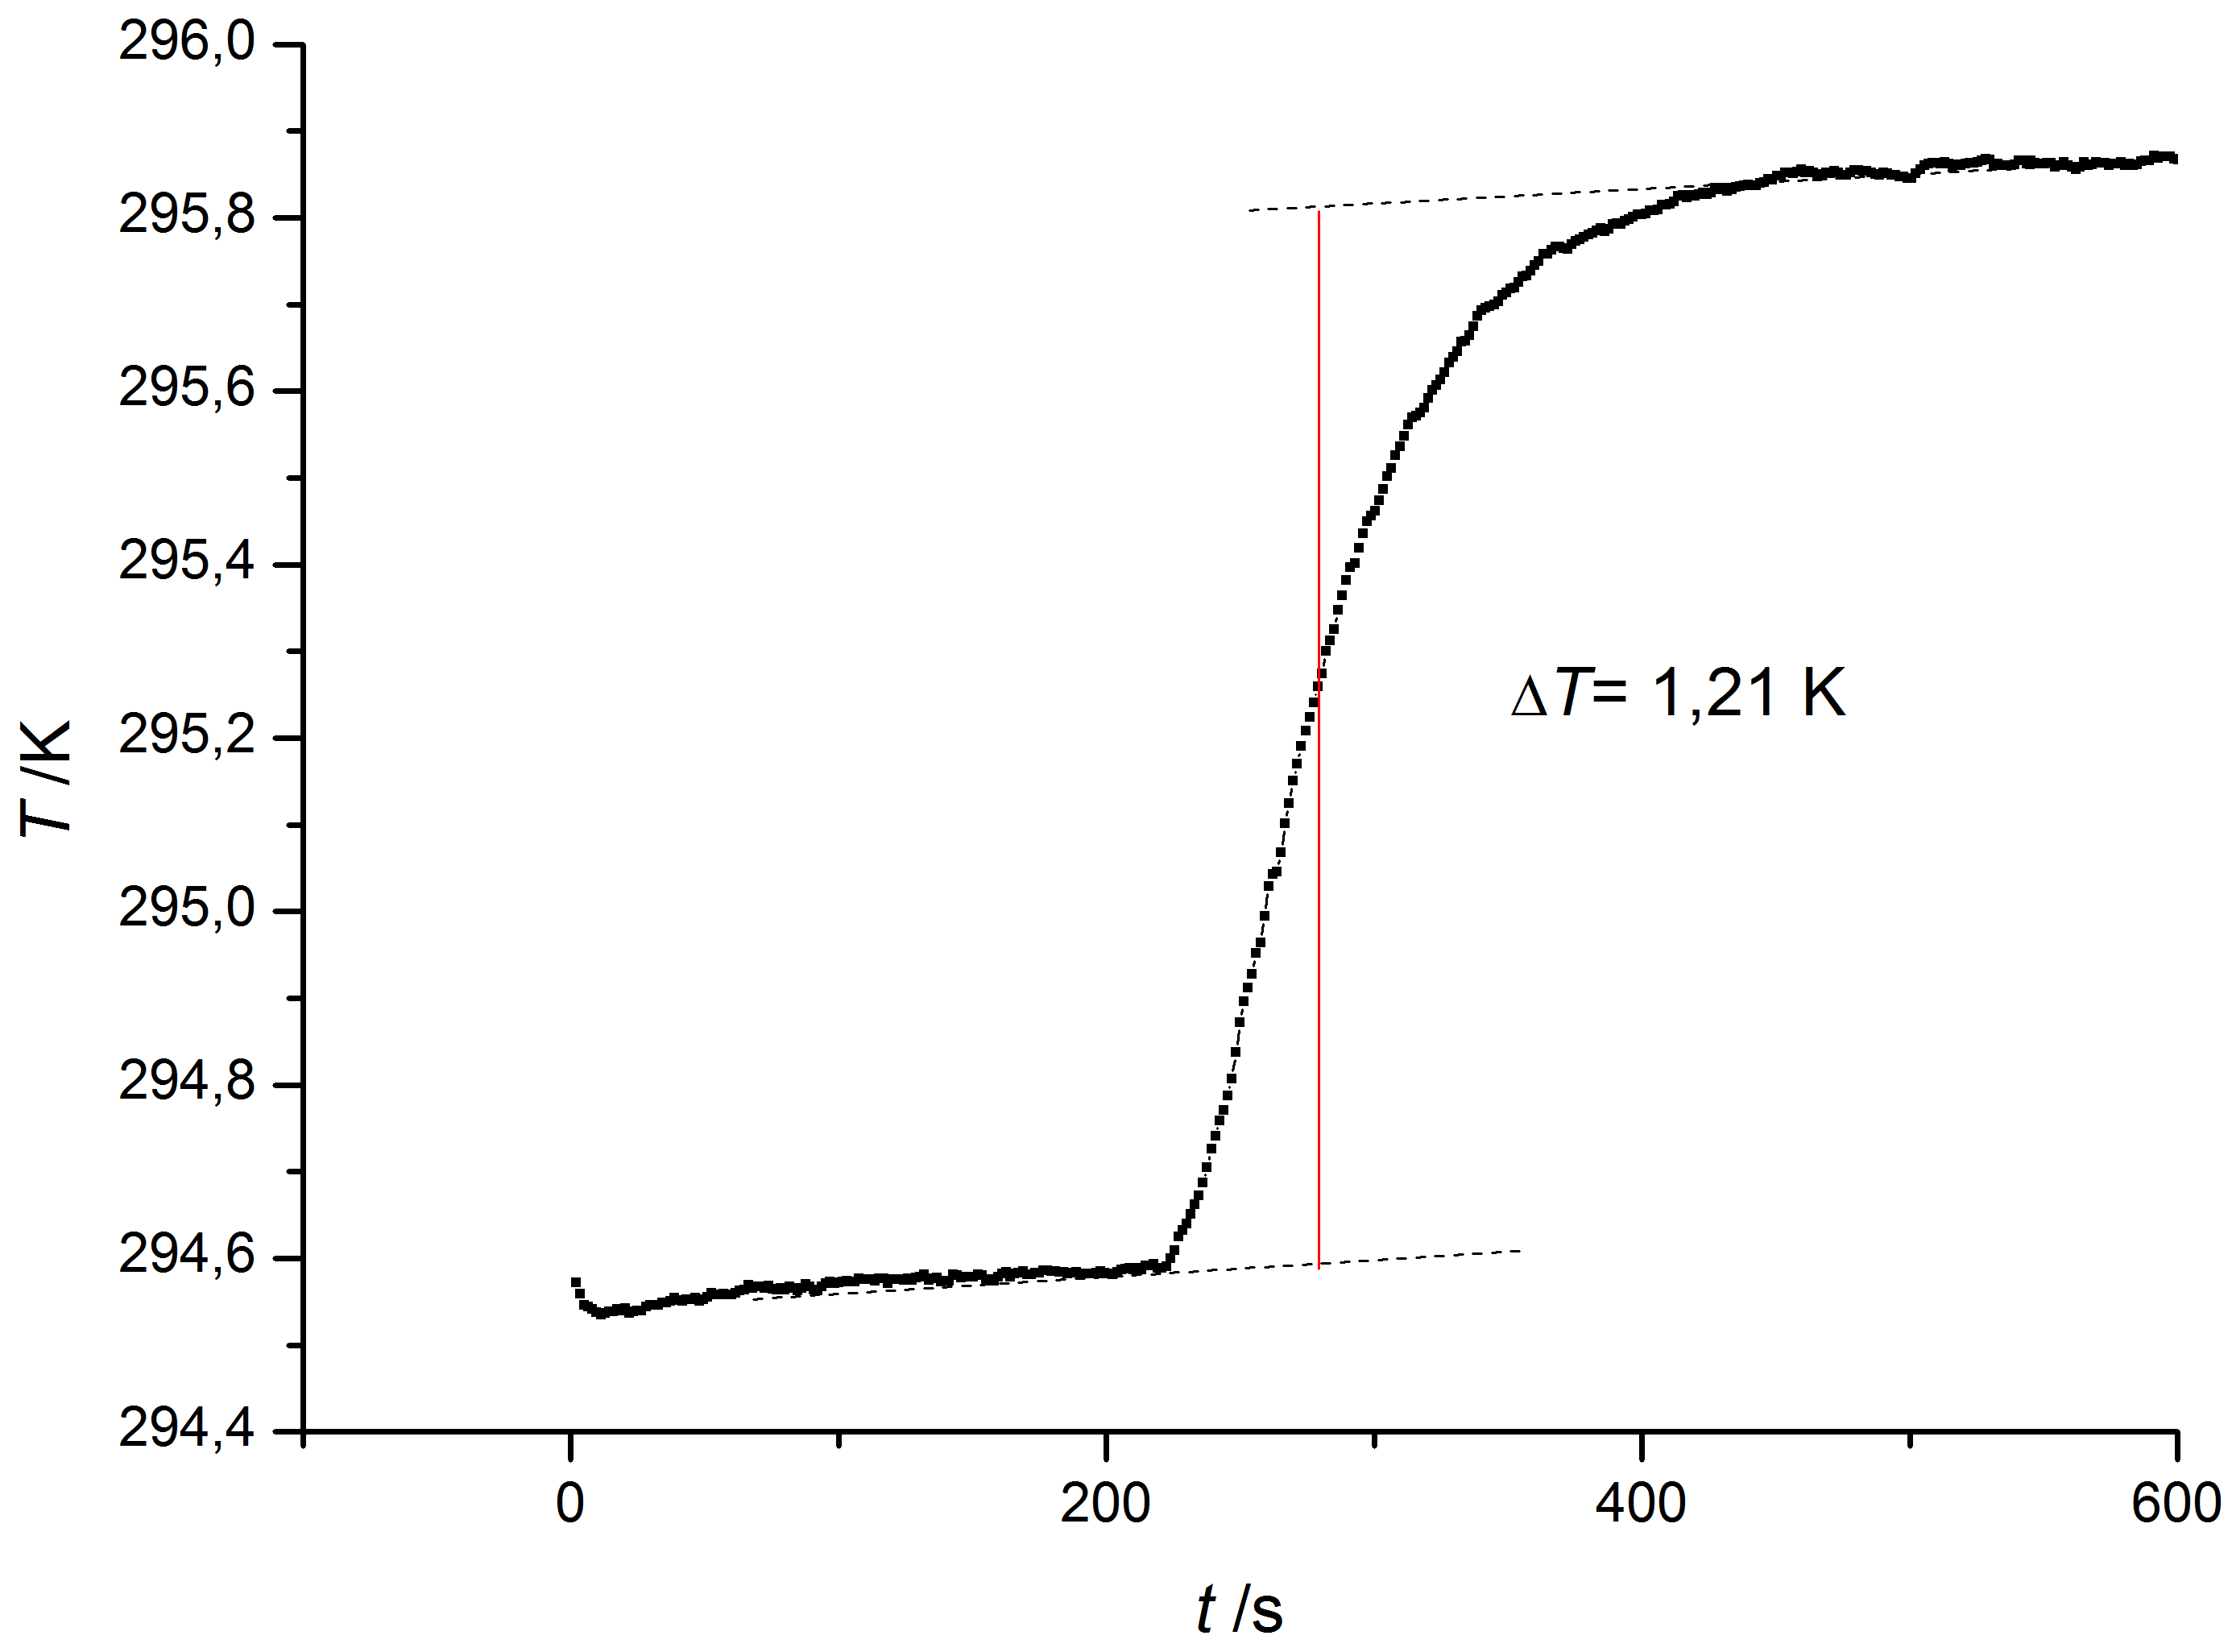
\includegraphics[scale=0.45]{Benz1.png} \end{center}
\caption{Benzoesäure Messung 1.}
\end{figure}

\begin{figure} [h!]
\begin{center}
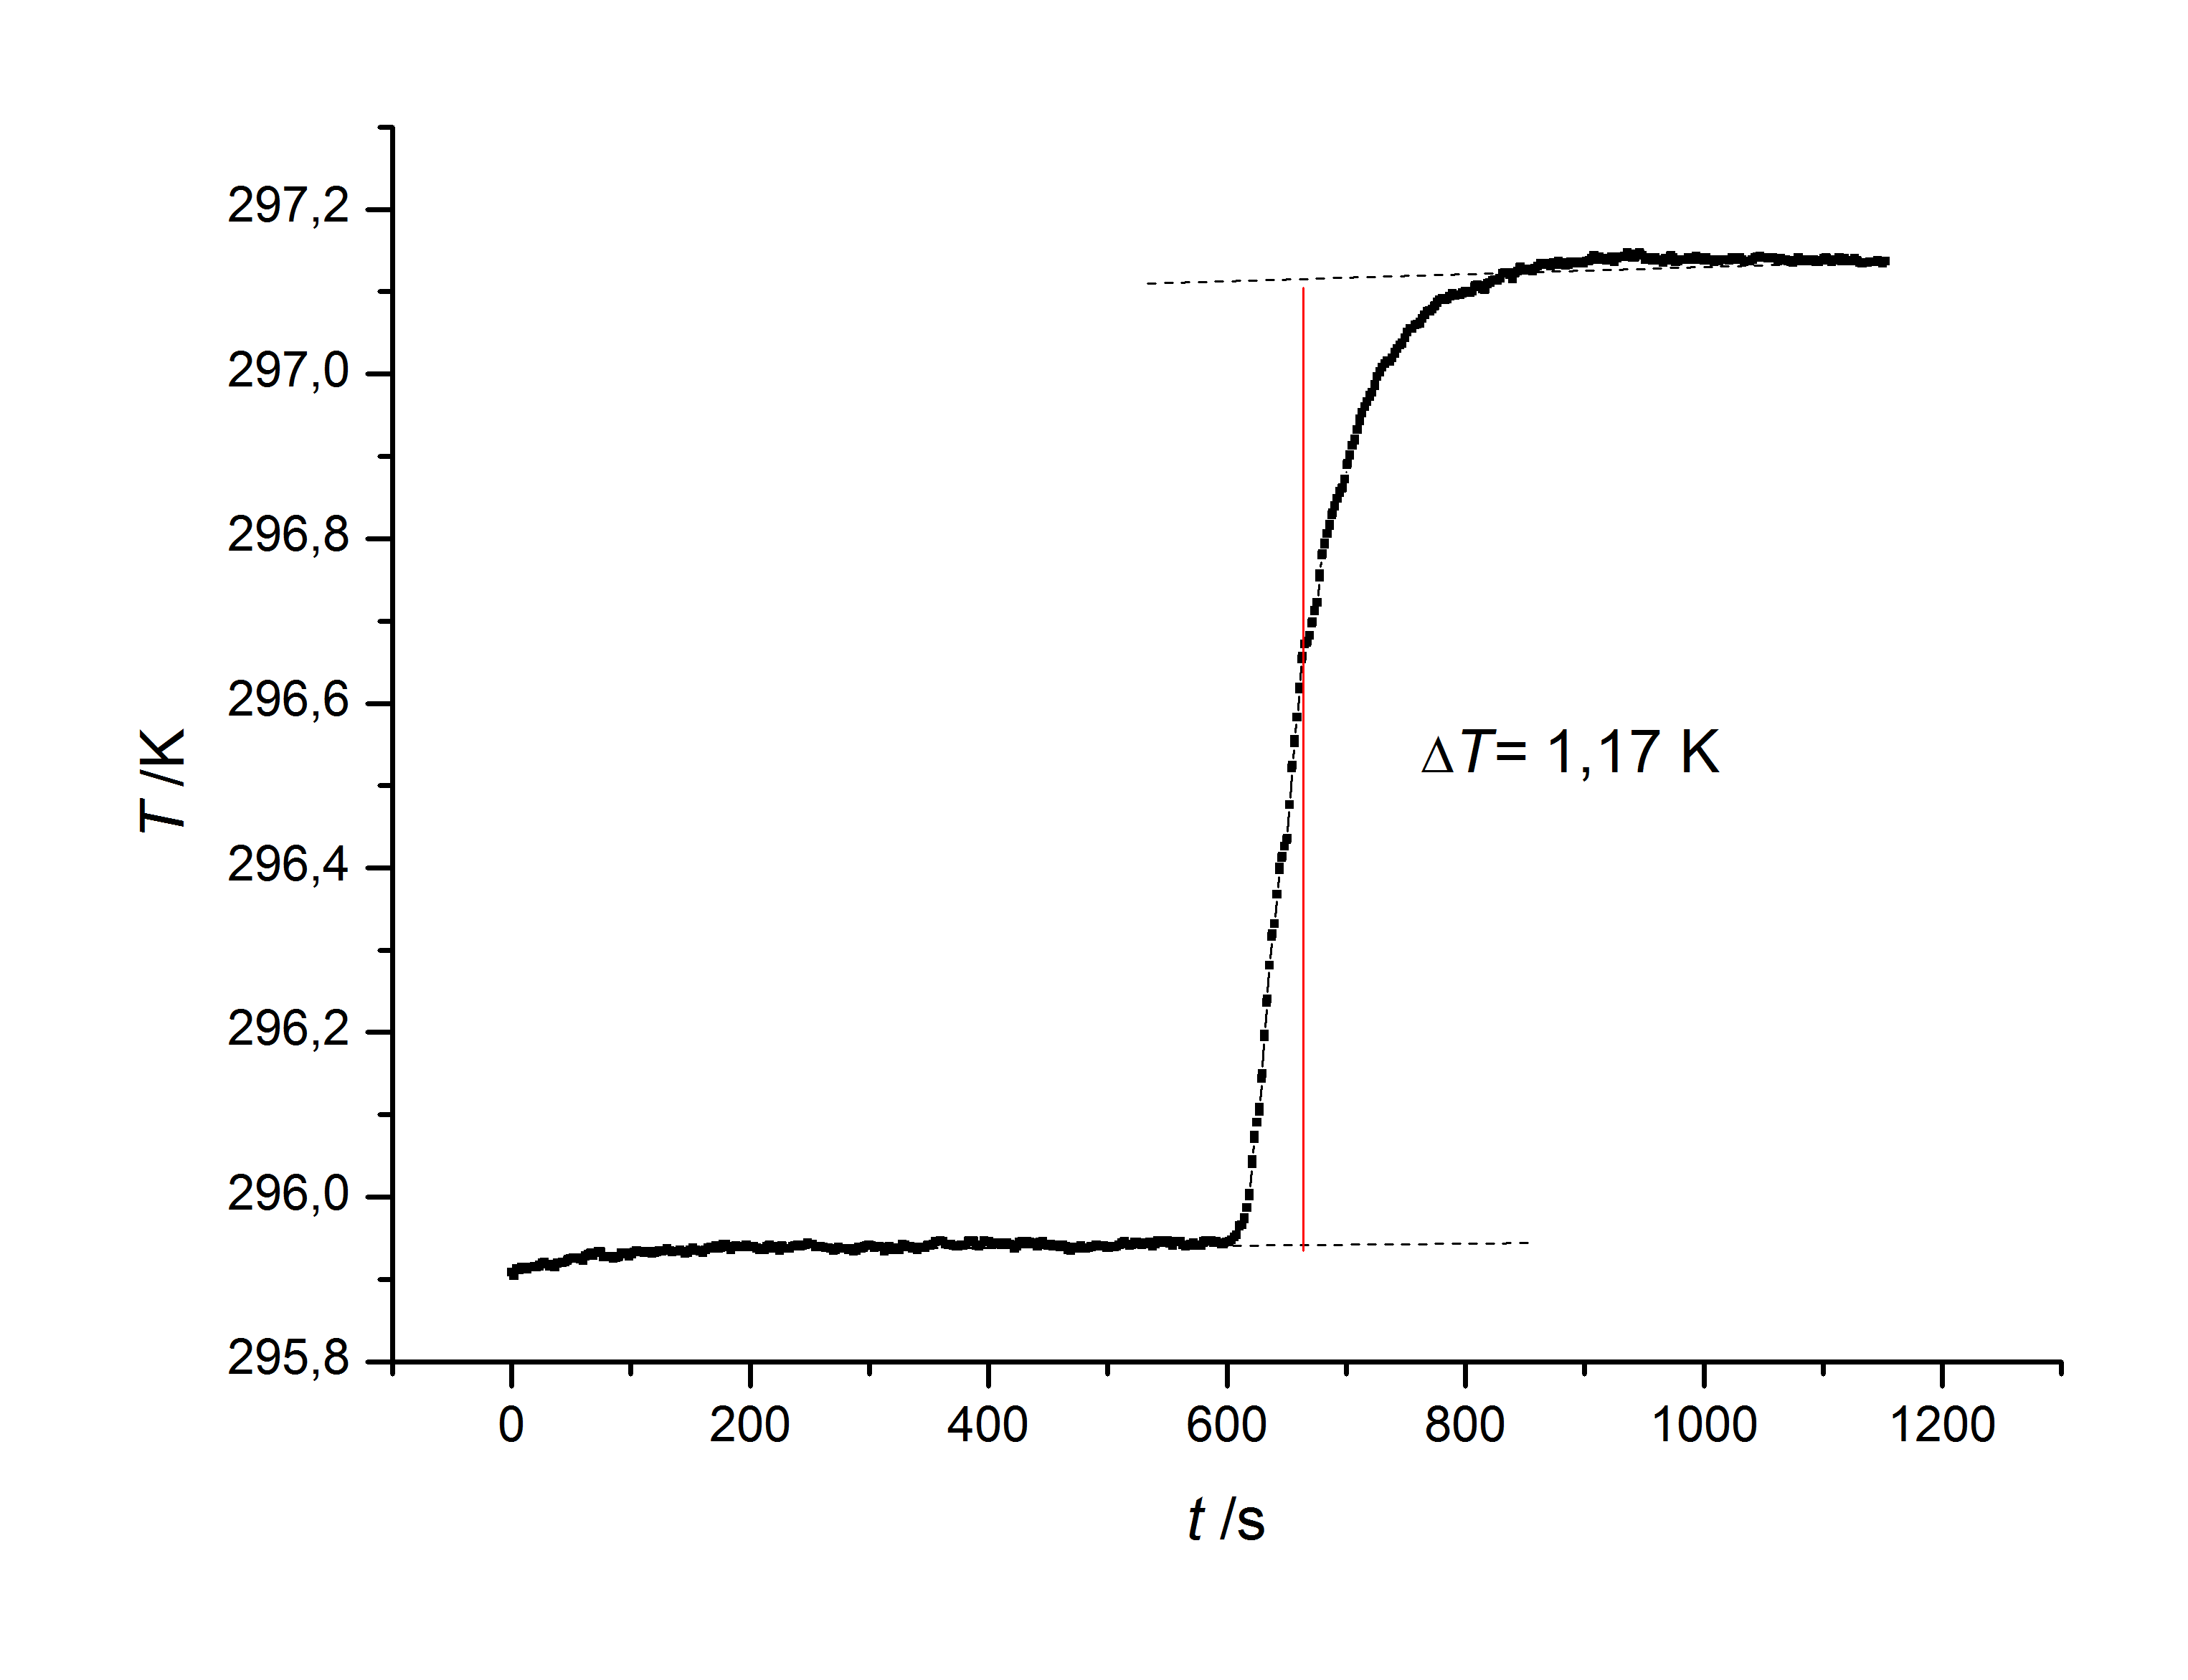
\includegraphics[scale=0.45]{Benz2.png} \end{center}
\caption{Benzoesäure Messung 2.}
\end{figure}

\begin{figure} [h!]
\begin{center}
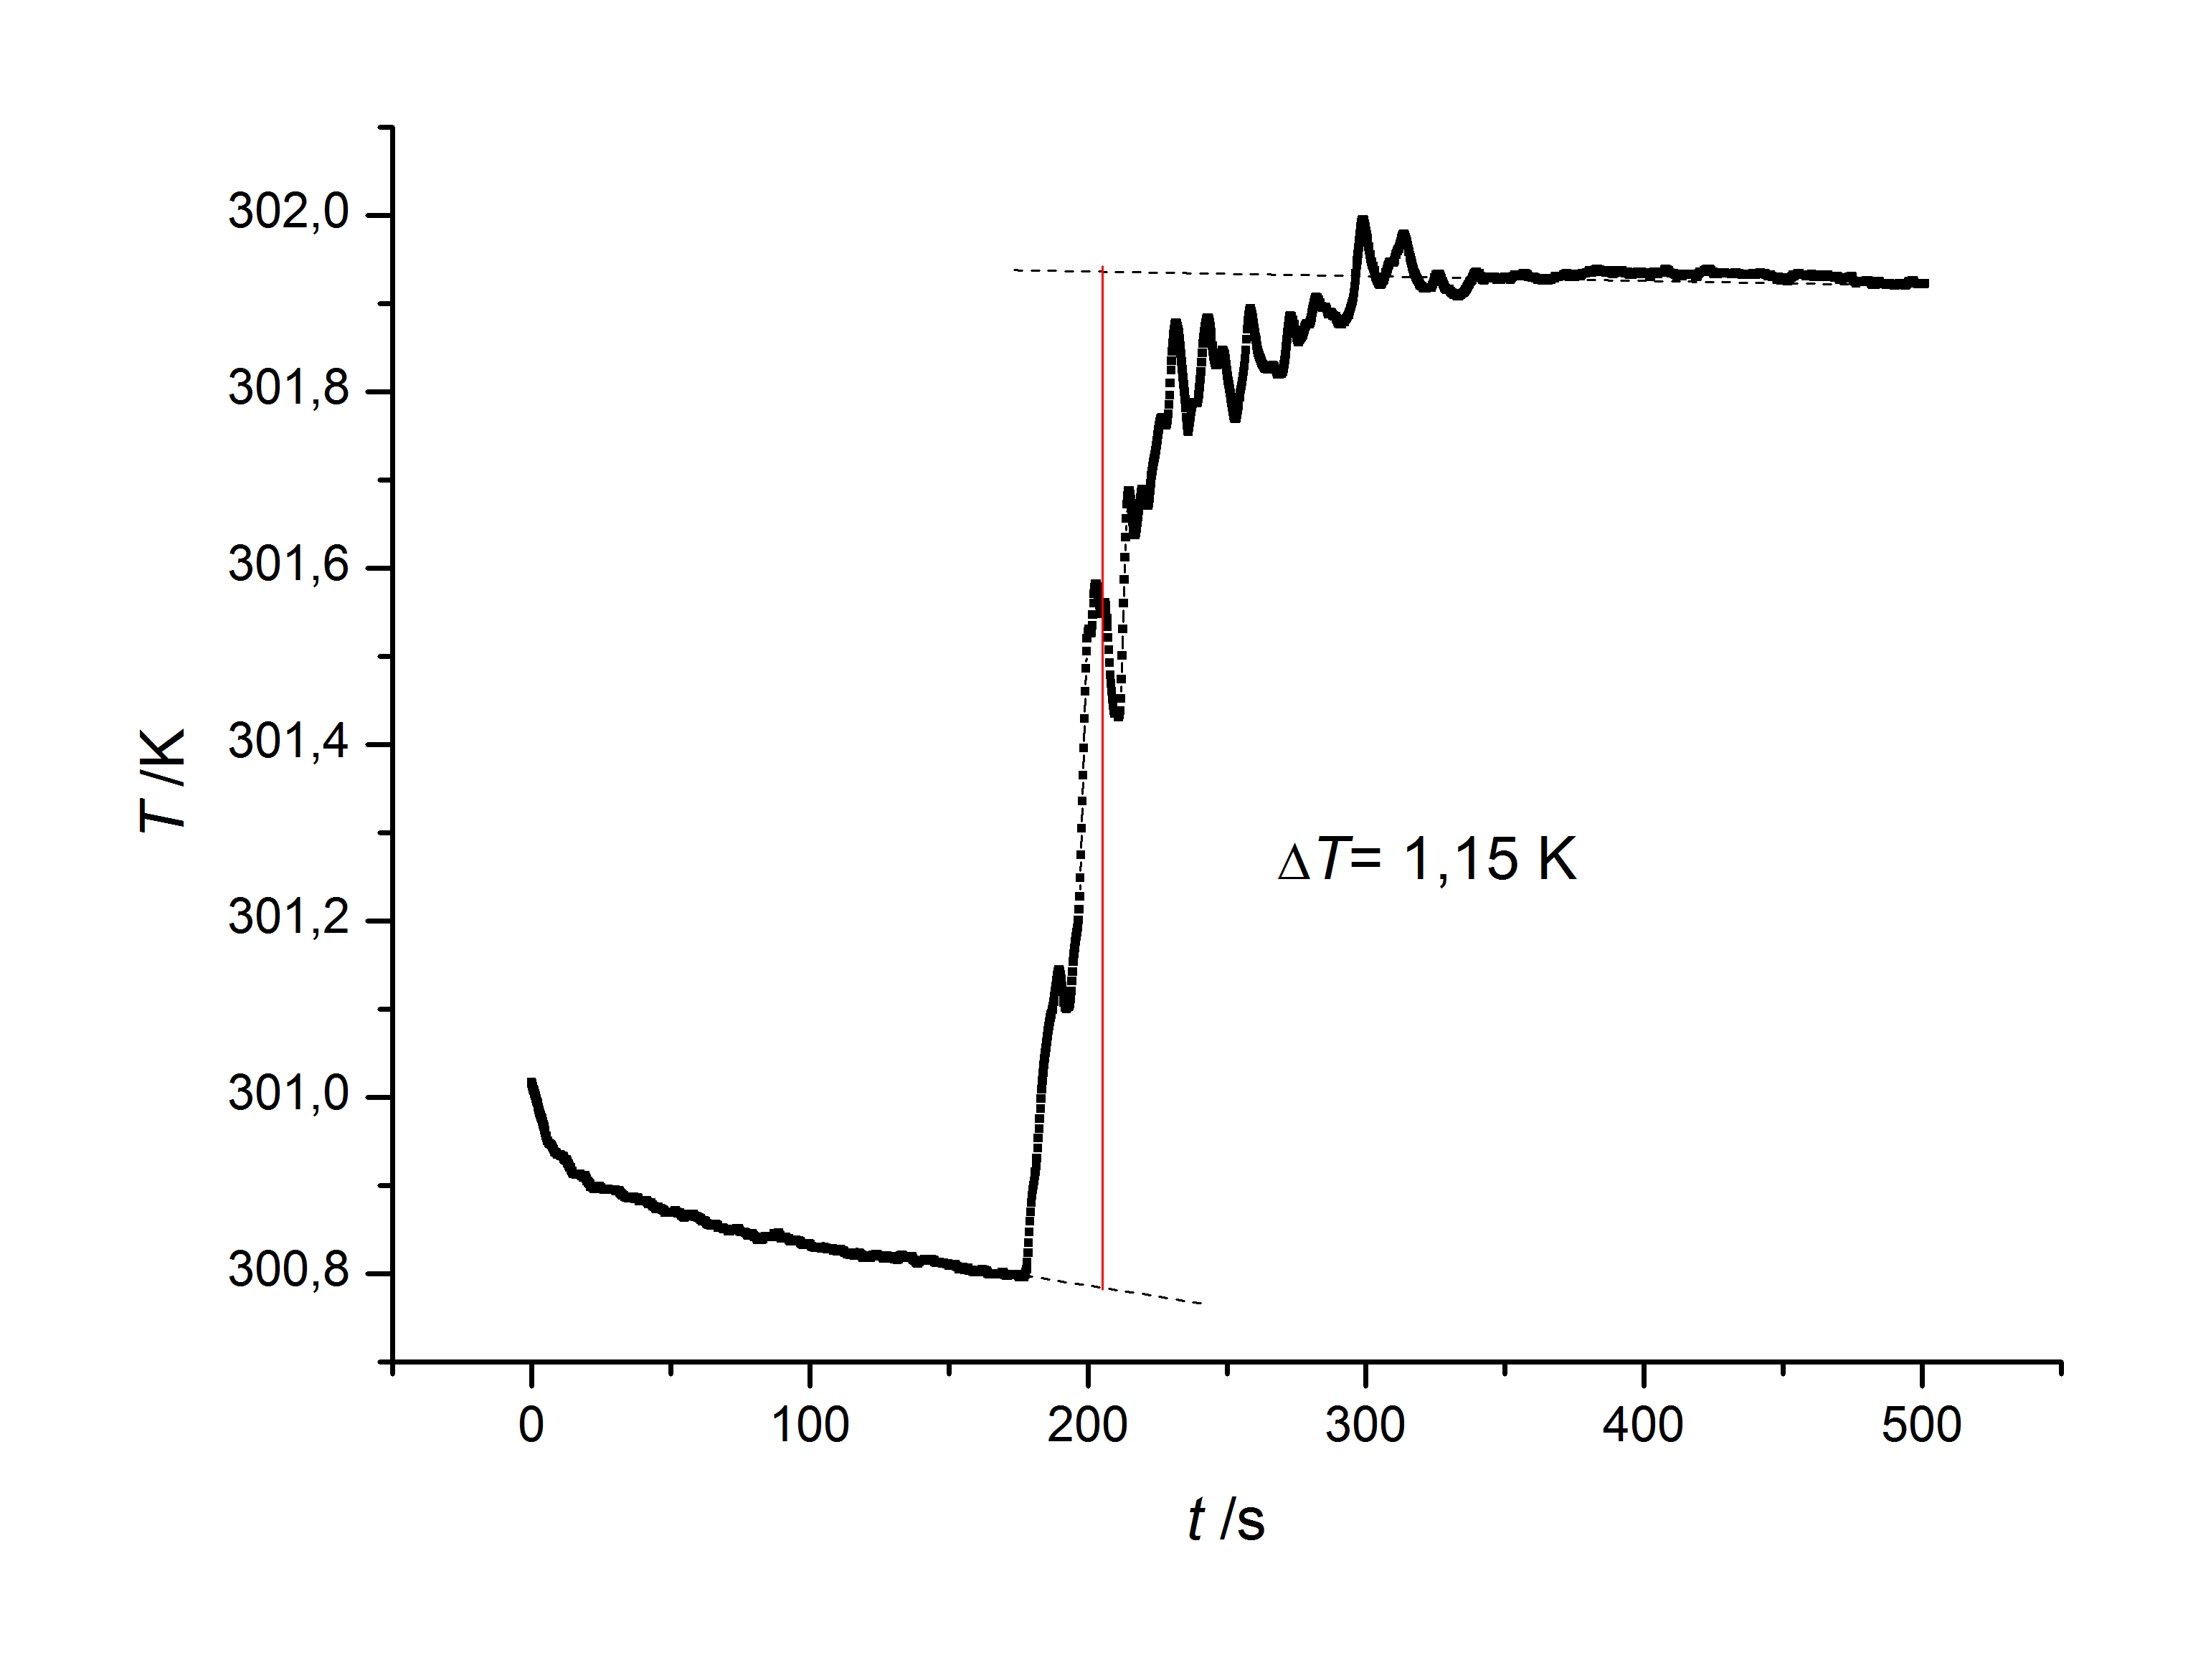
\includegraphics[scale=0.45]{Benz3.png} \end{center}
\caption{Benzoesäure Messung 3.}
\end{figure}

\begin{figure} [h!]
\begin{center}
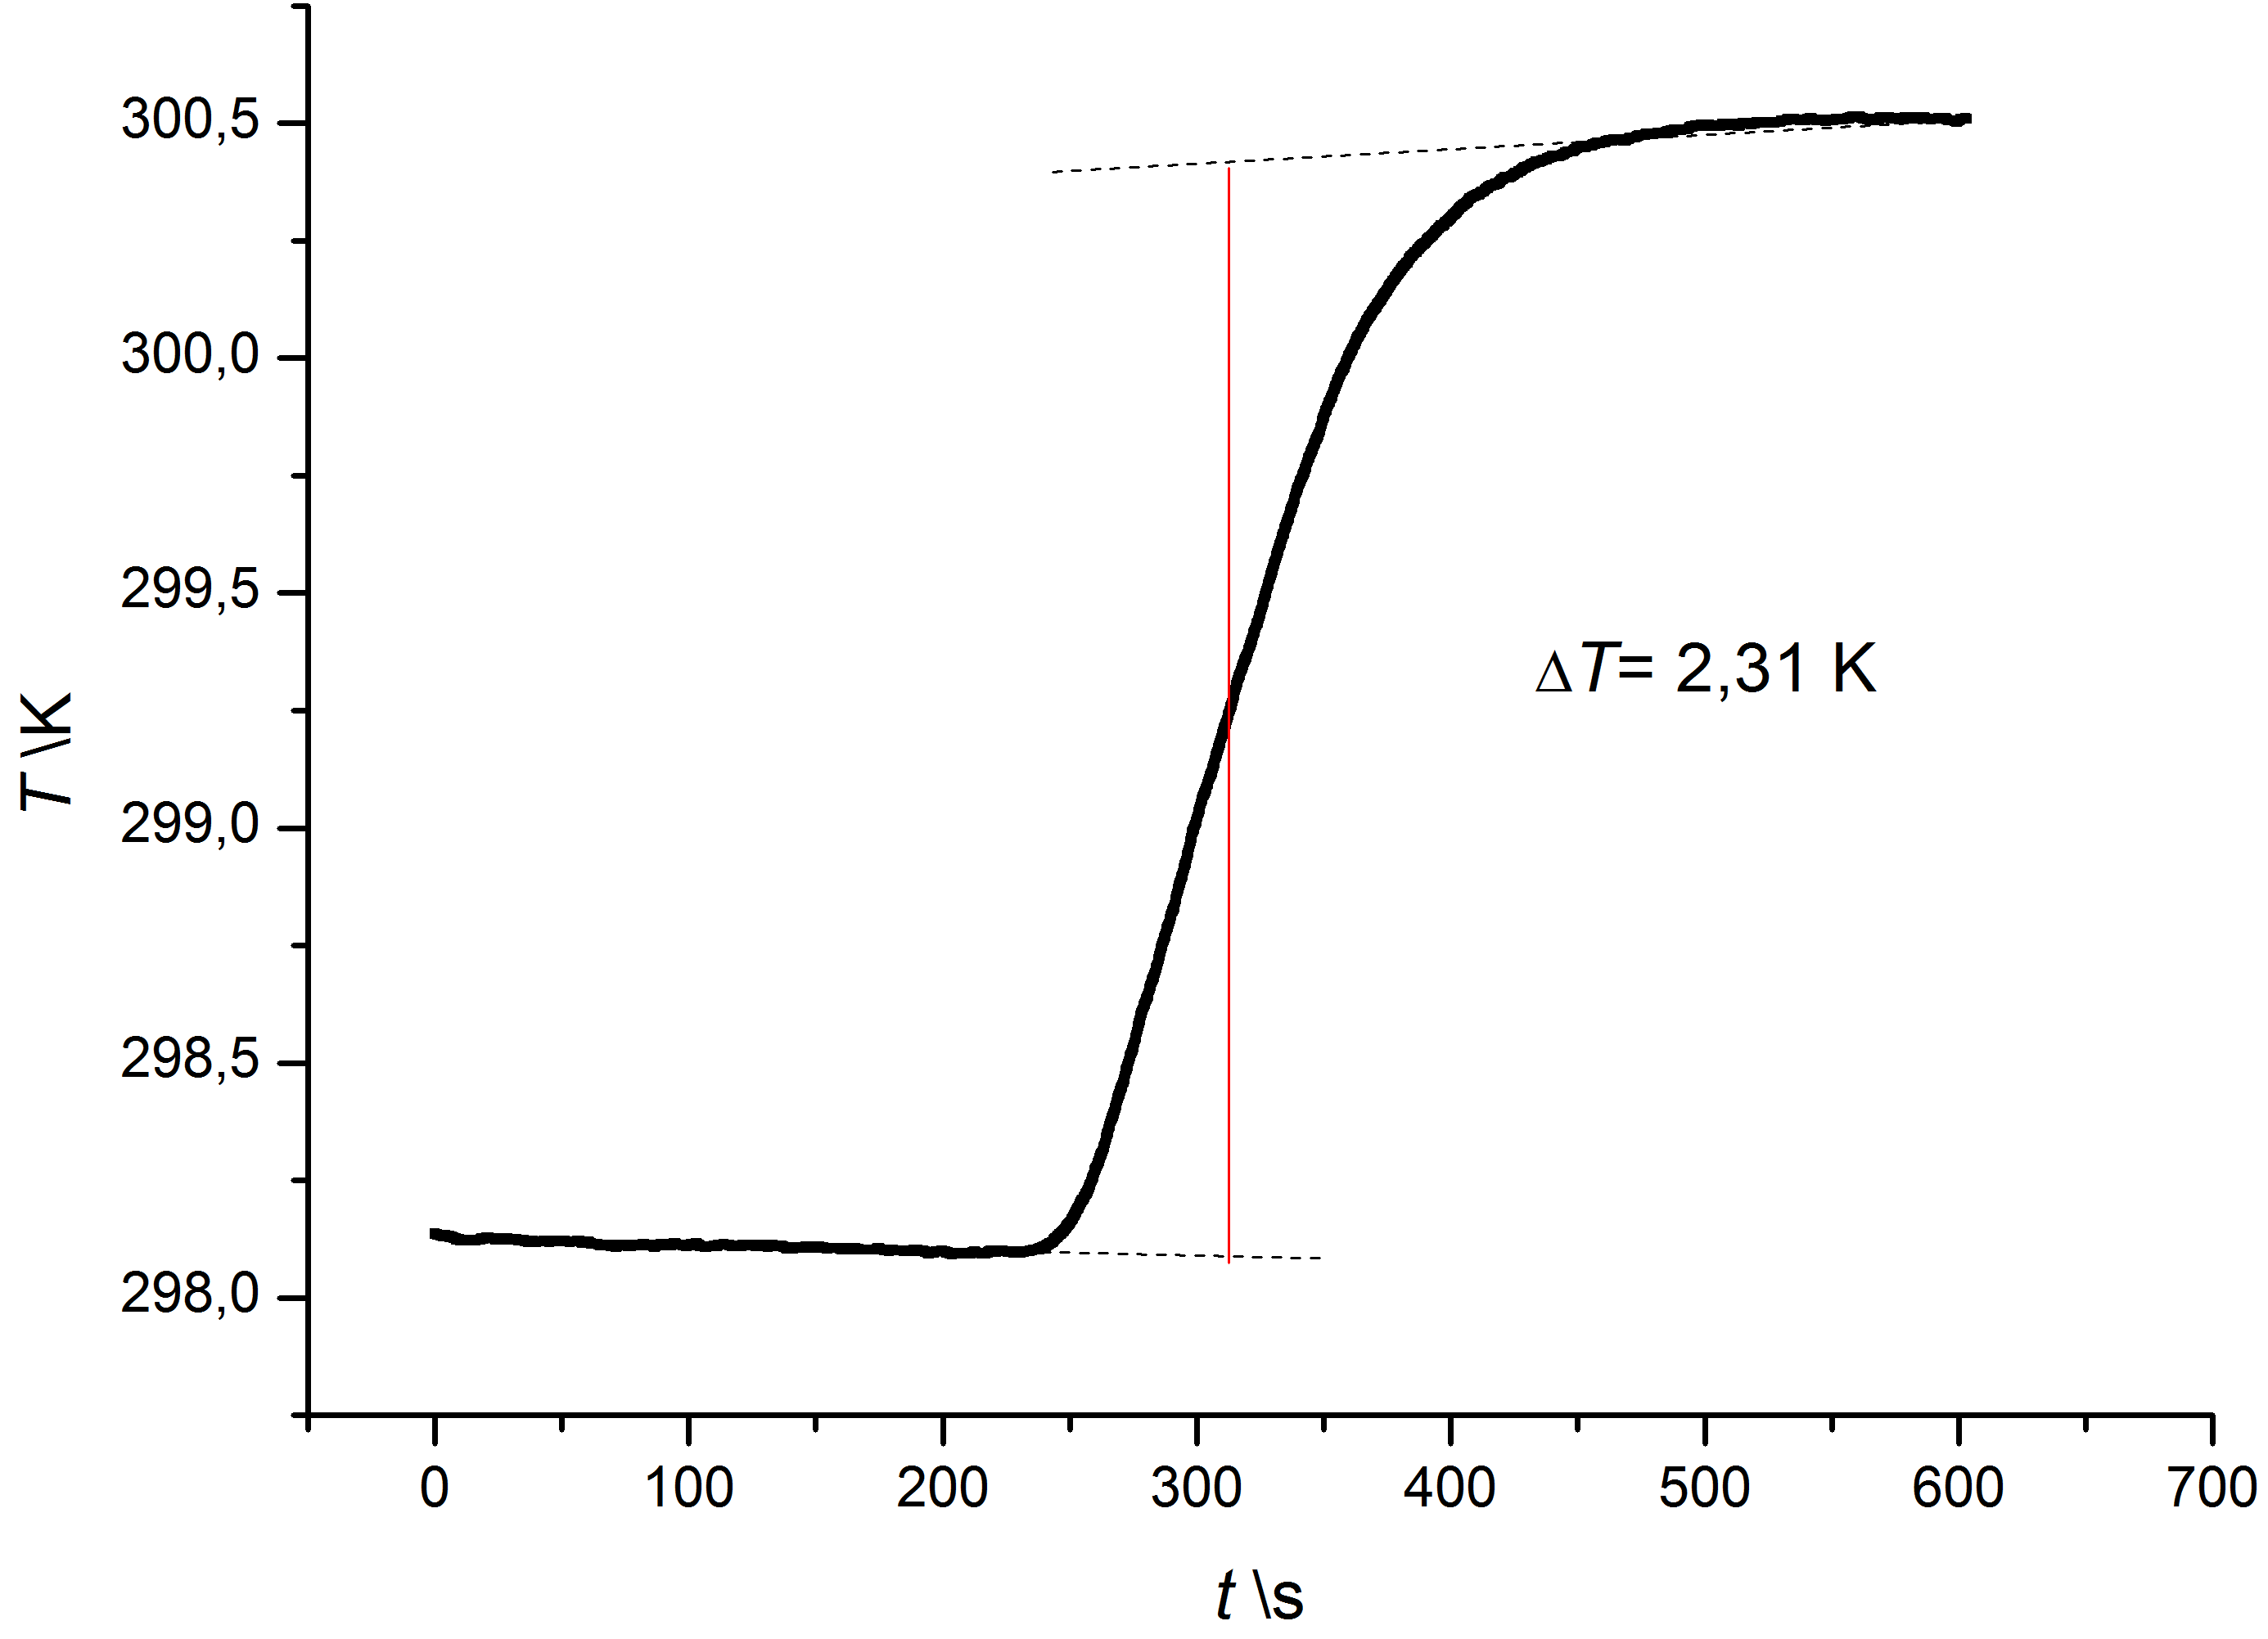
\includegraphics[scale=0.45]{Napht1.png} \end{center}
\caption{Naphthalin Messung 1.}
\end{figure}

\begin{figure} [h!]
\begin{center}
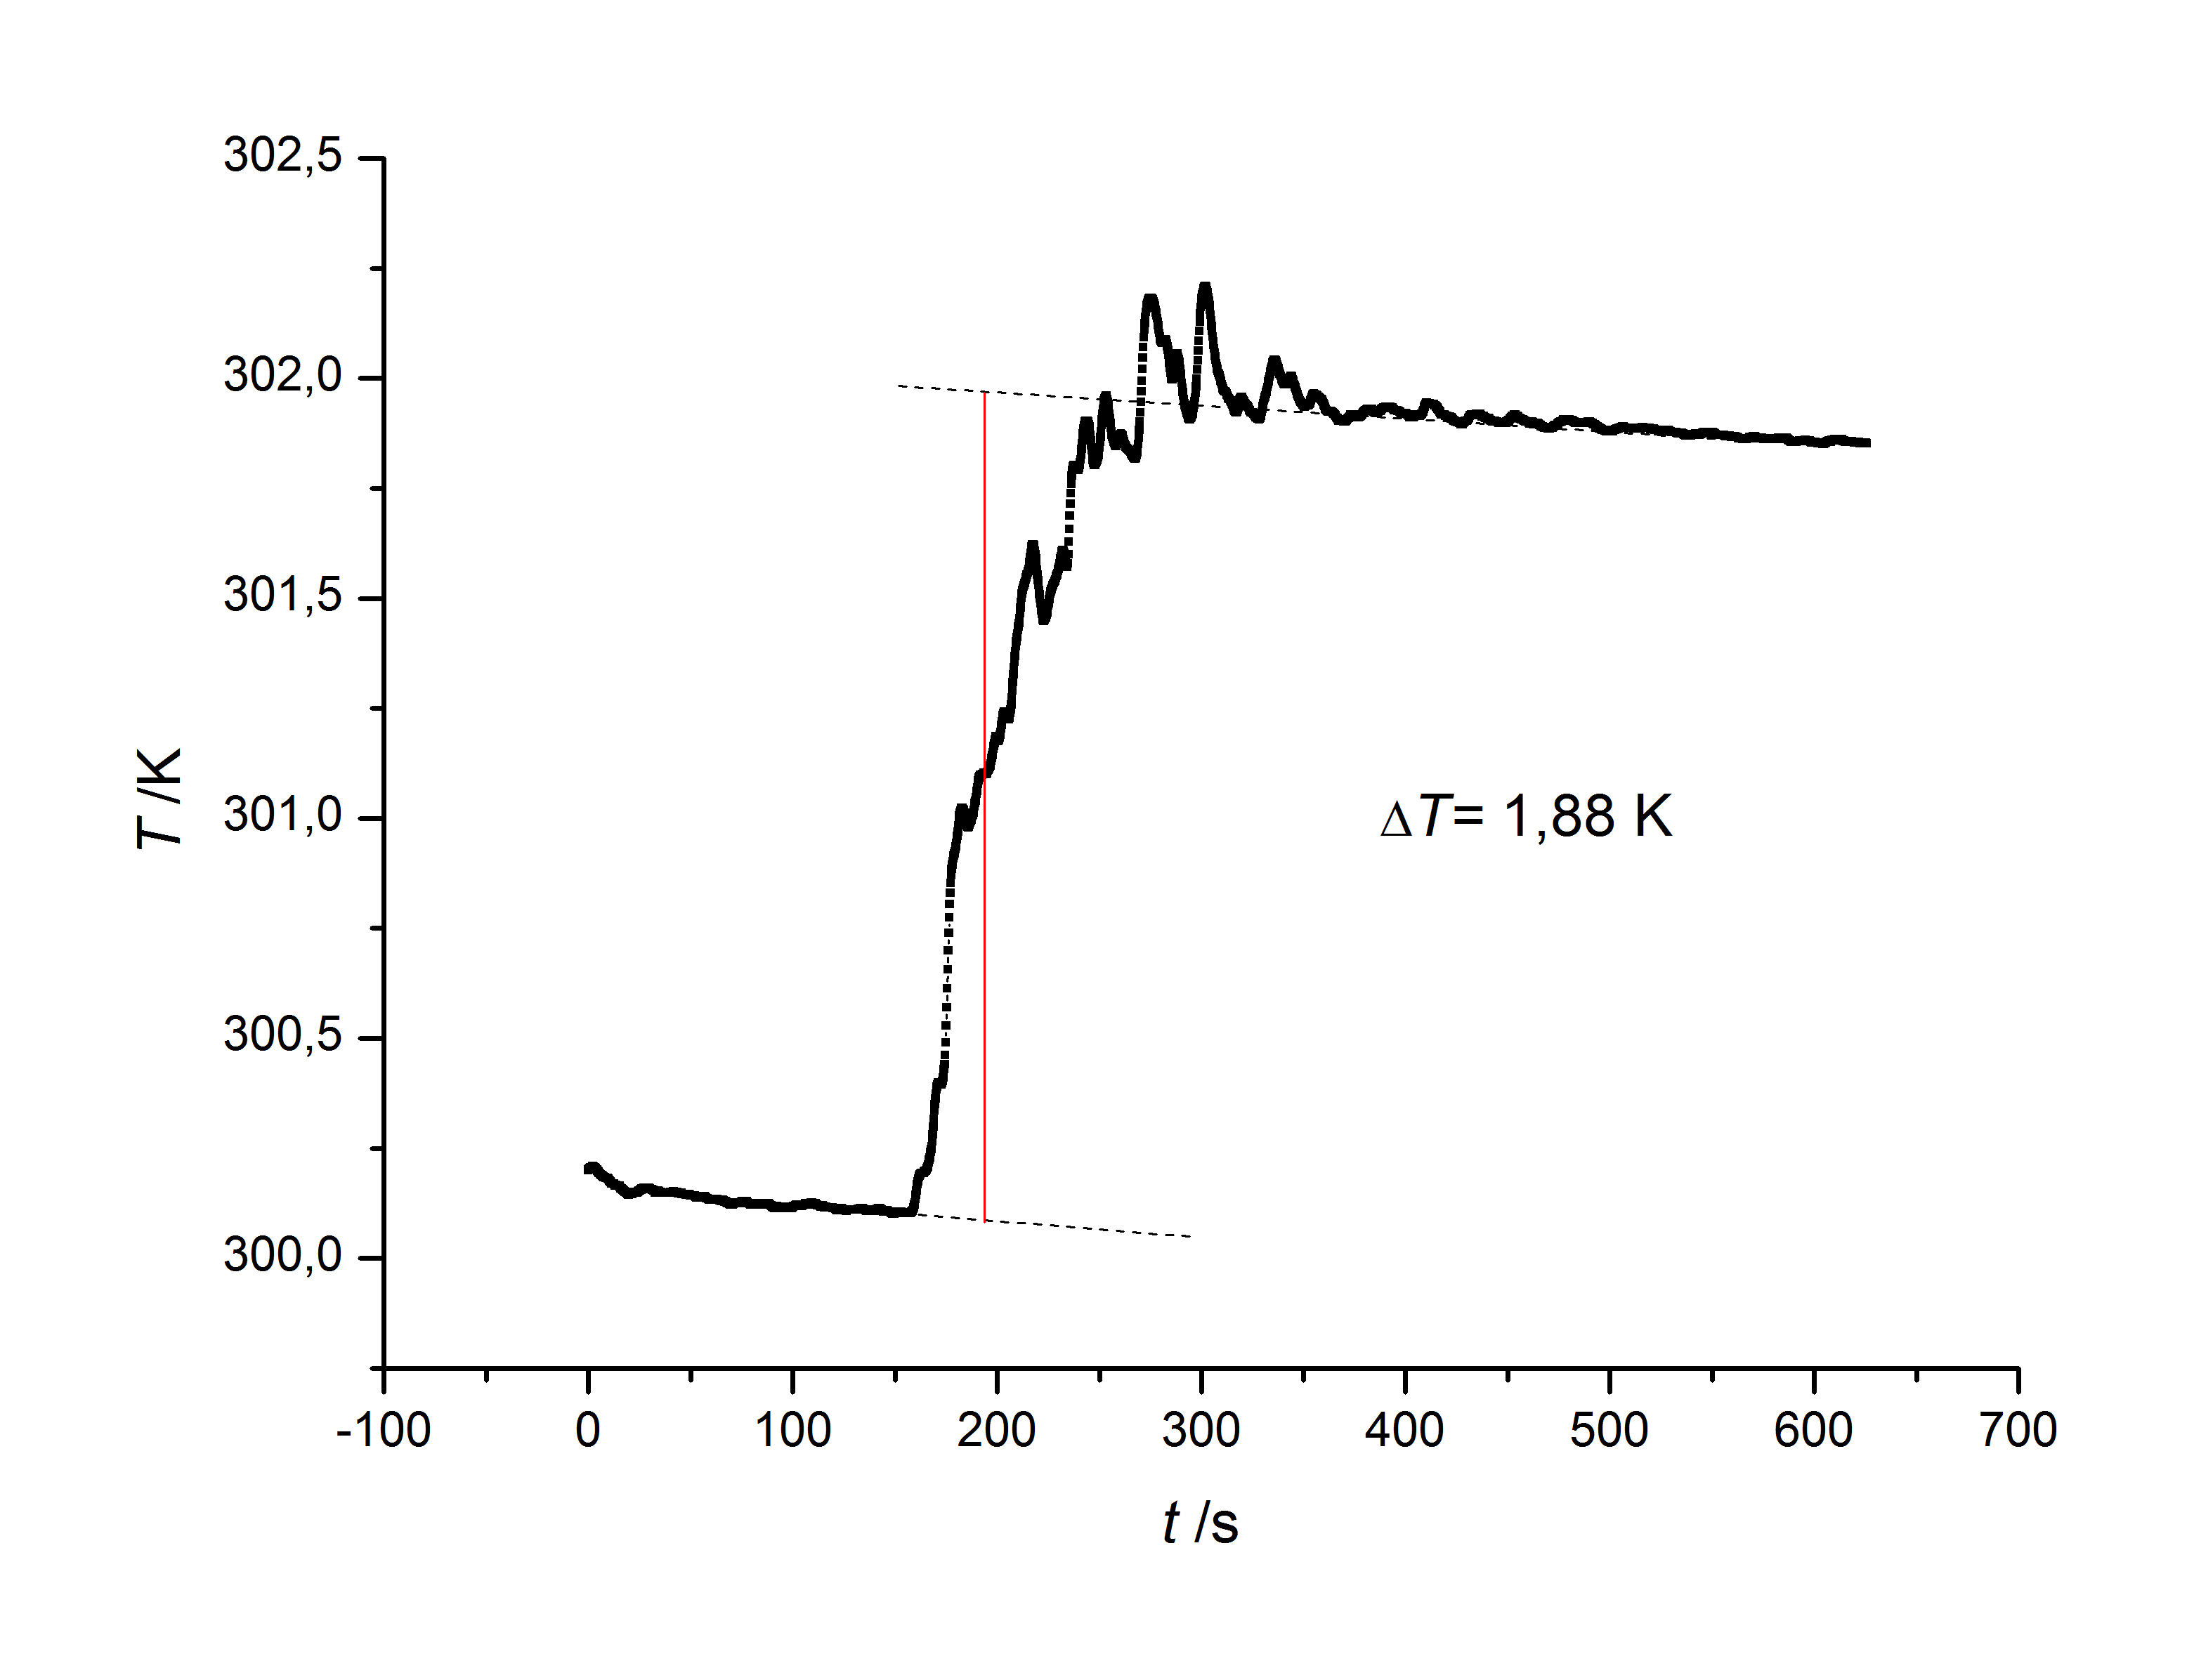
\includegraphics[scale=0.45]{Napht2.png} \end{center}
\caption{Naphthalin Messung 2.}
\end{figure}

\begin{figure} [h!]
\begin{center}
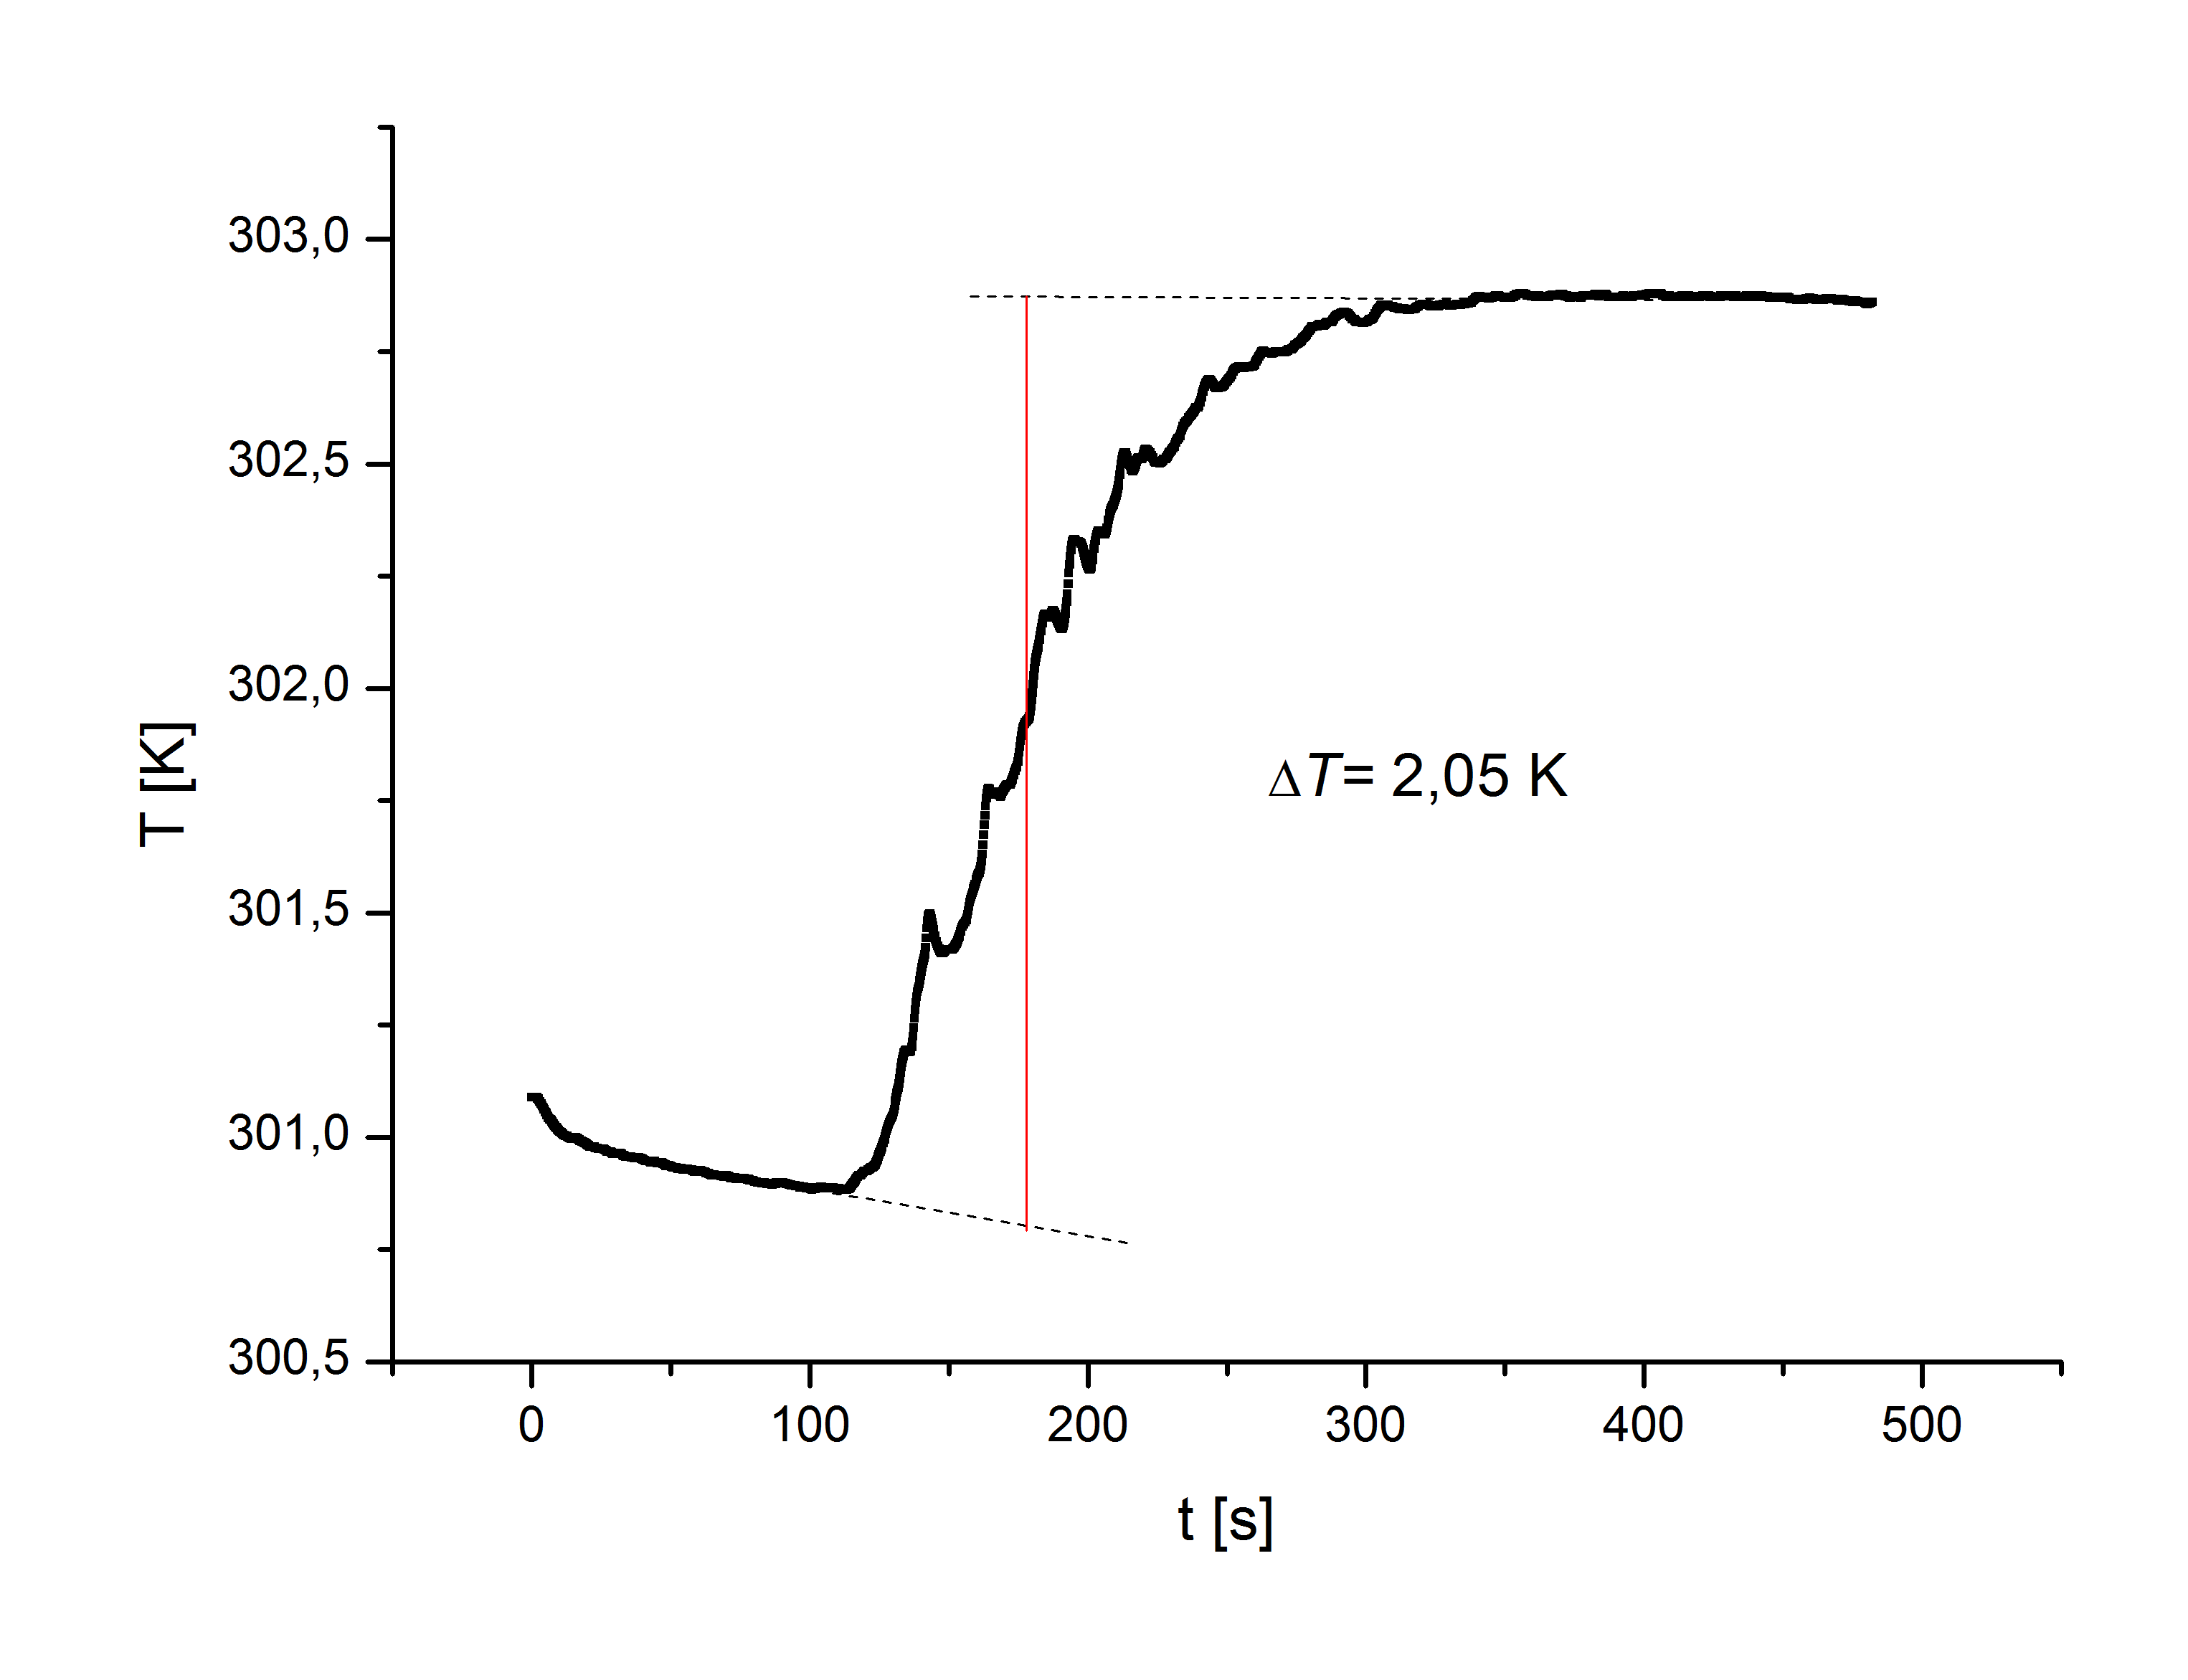
\includegraphics[scale=0.45]{Napht3.png} \end{center}
\caption{Naphthalin Messung 3.}
\end{figure}
\FloatBarrier

\subsection{Auftragungen mit Grenzgeraden}
\begin{figure} [h!]
\begin{center}
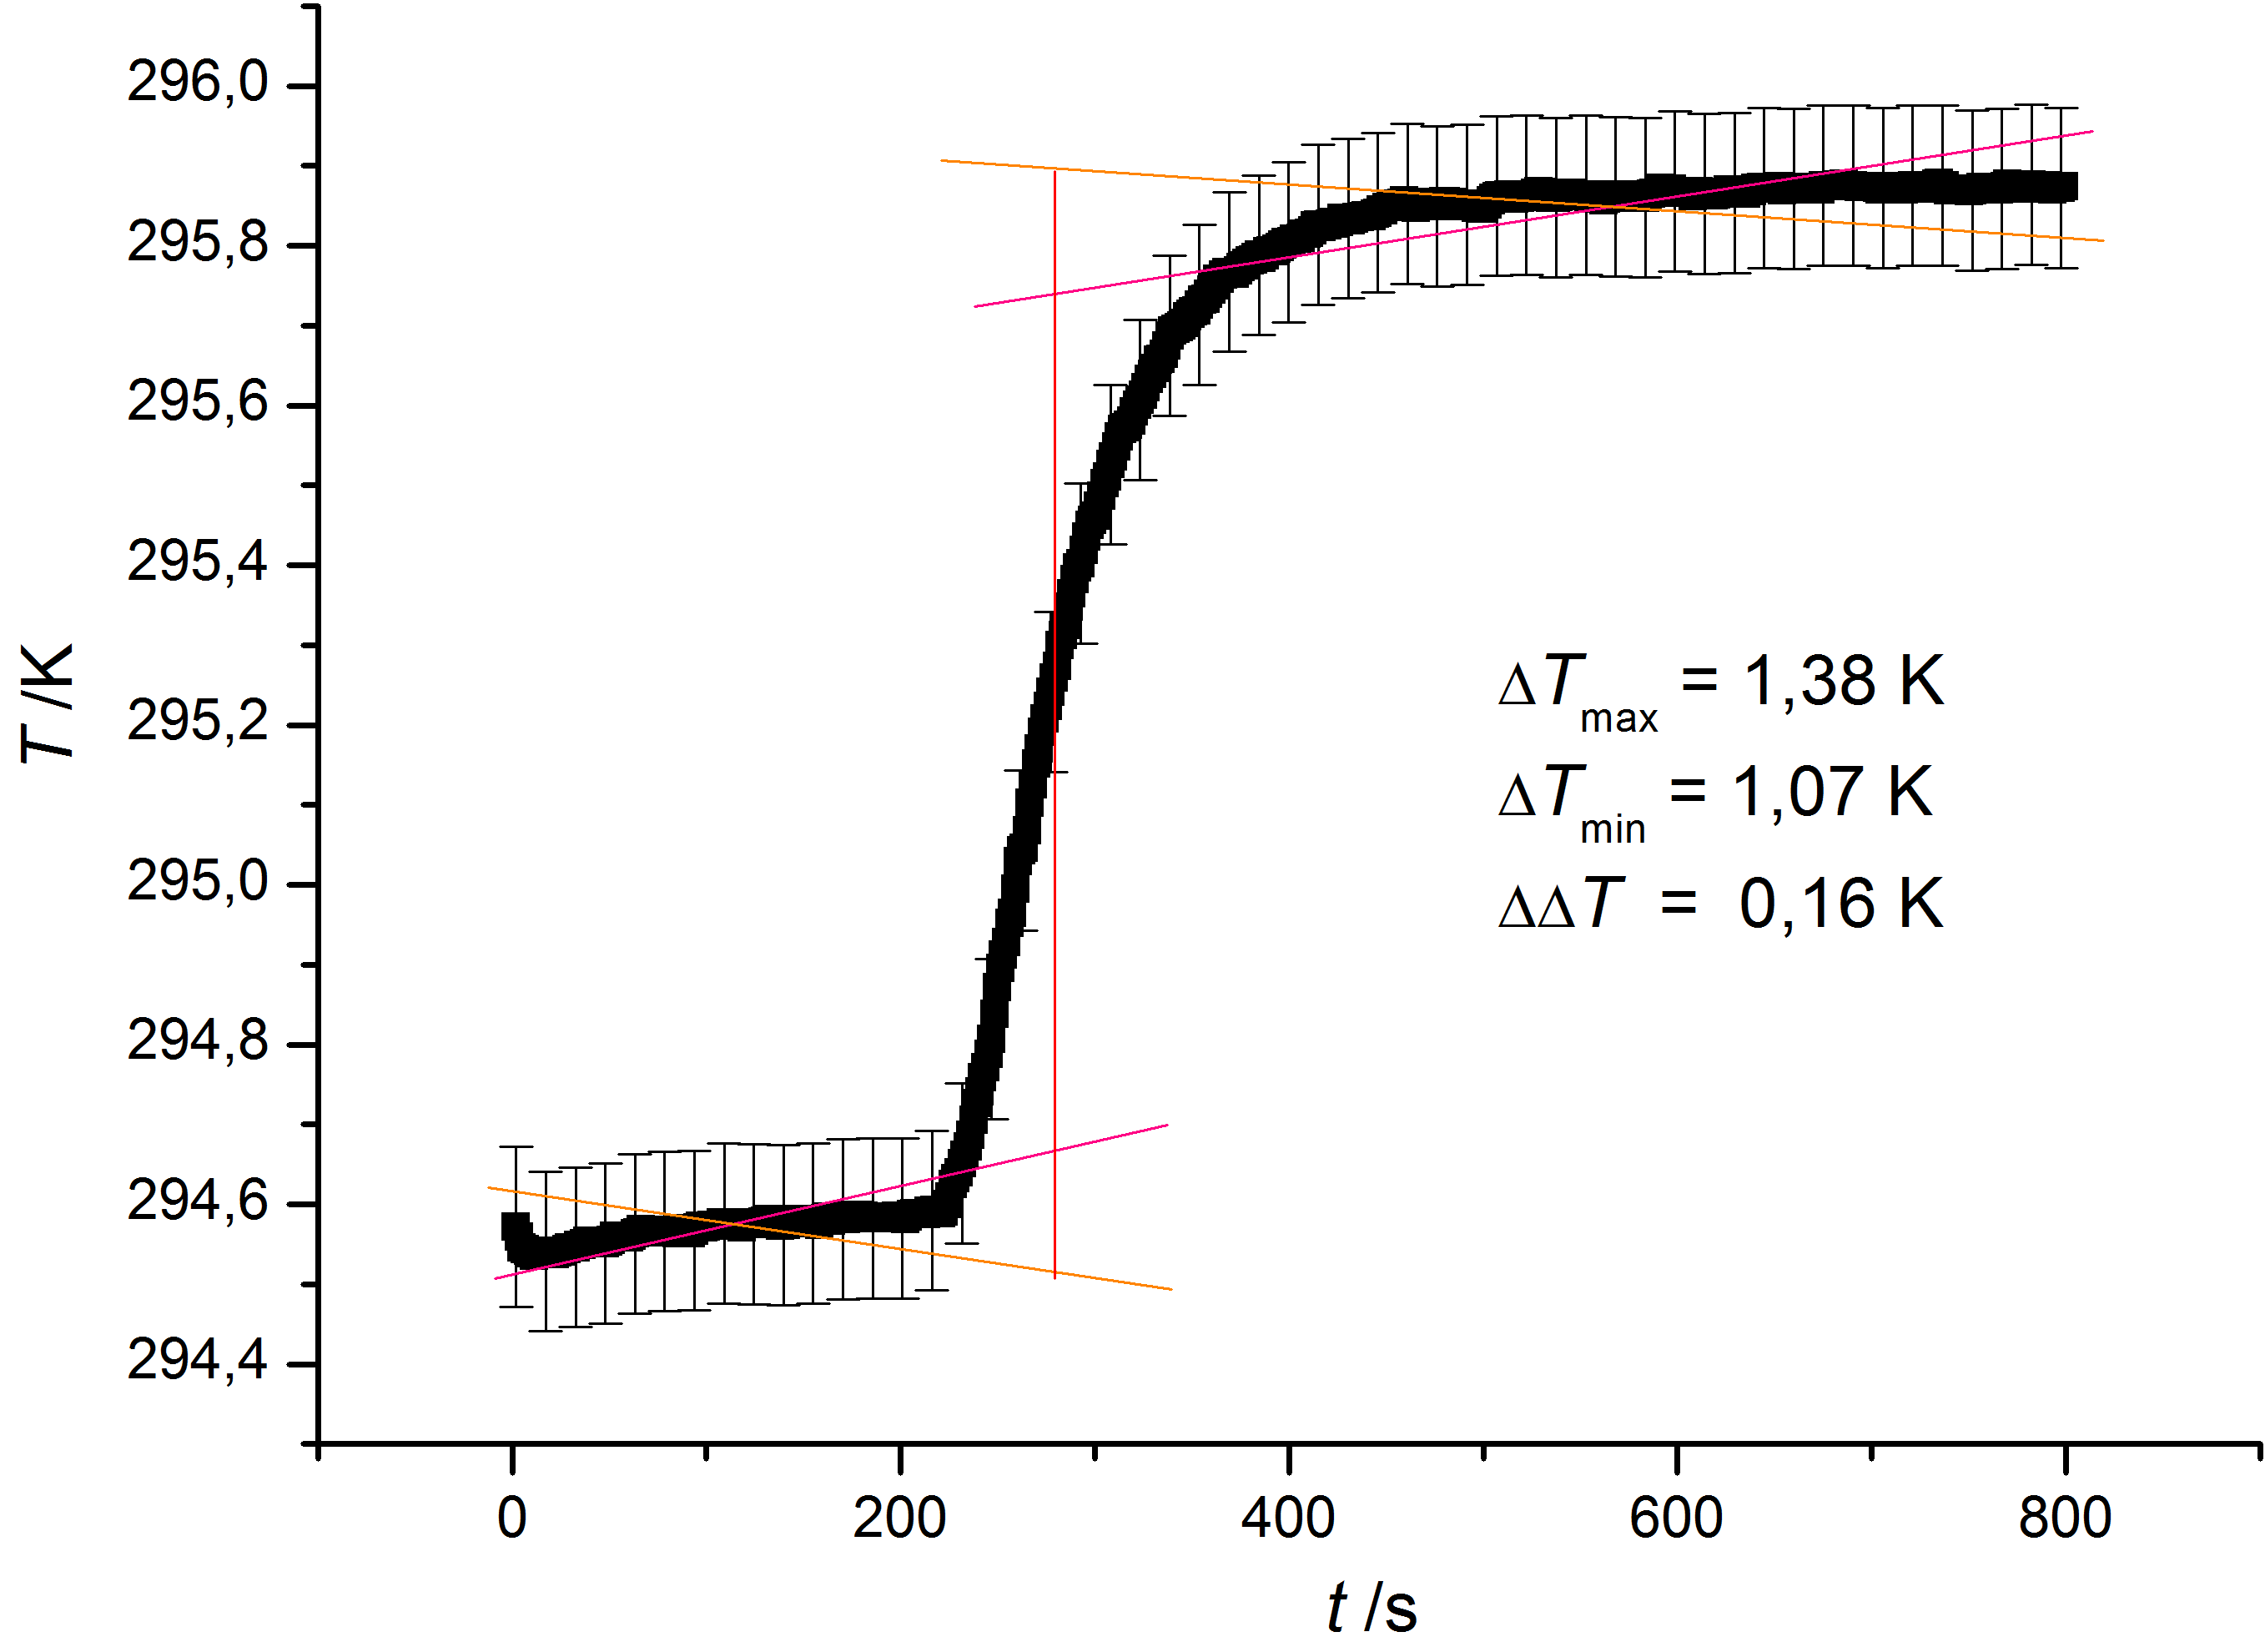
\includegraphics[scale=0.45]{Benz1Fehler.png} \end{center}
\caption{Benzoesäure Messung 1 mit Grenzgeraden.}
\end{figure}

\begin{figure} [h!]
\begin{center}
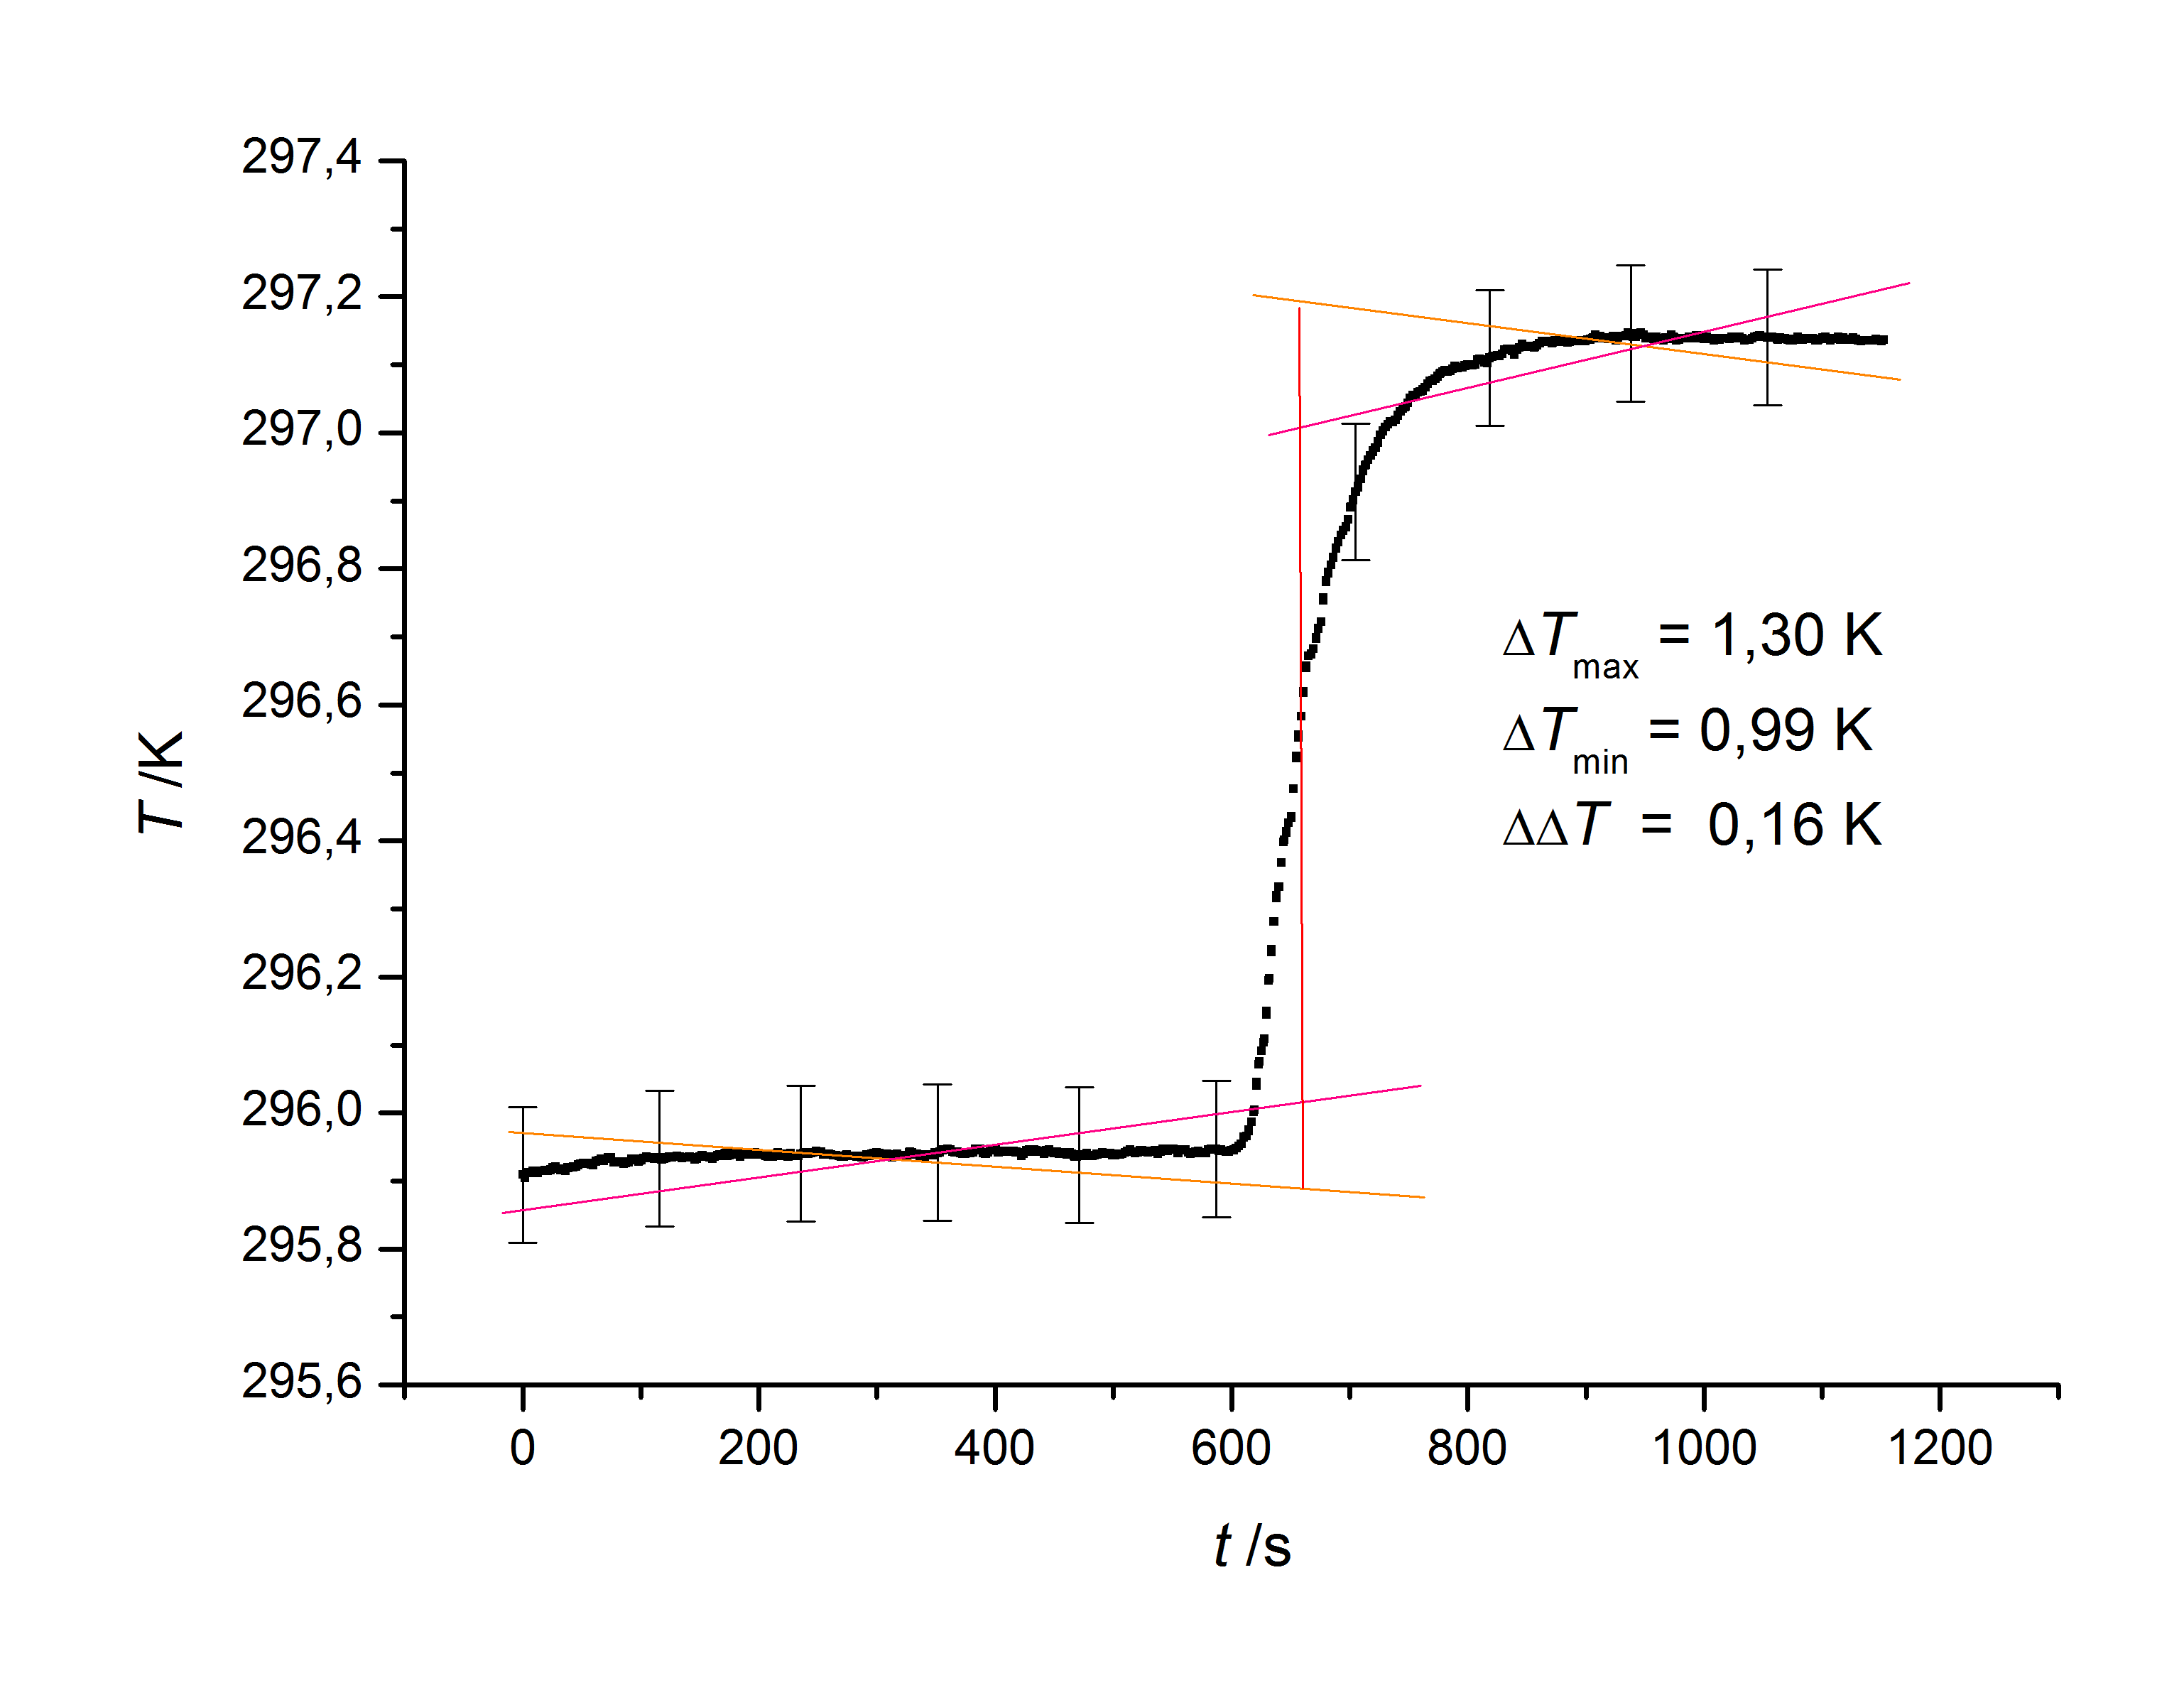
\includegraphics[scale=0.45]{Benz2Fehler.png} \end{center}
\caption{Benzoesäure Messung 2 mit Grenzgeraden.}
\end{figure}

\begin{figure} [h!]
\begin{center}
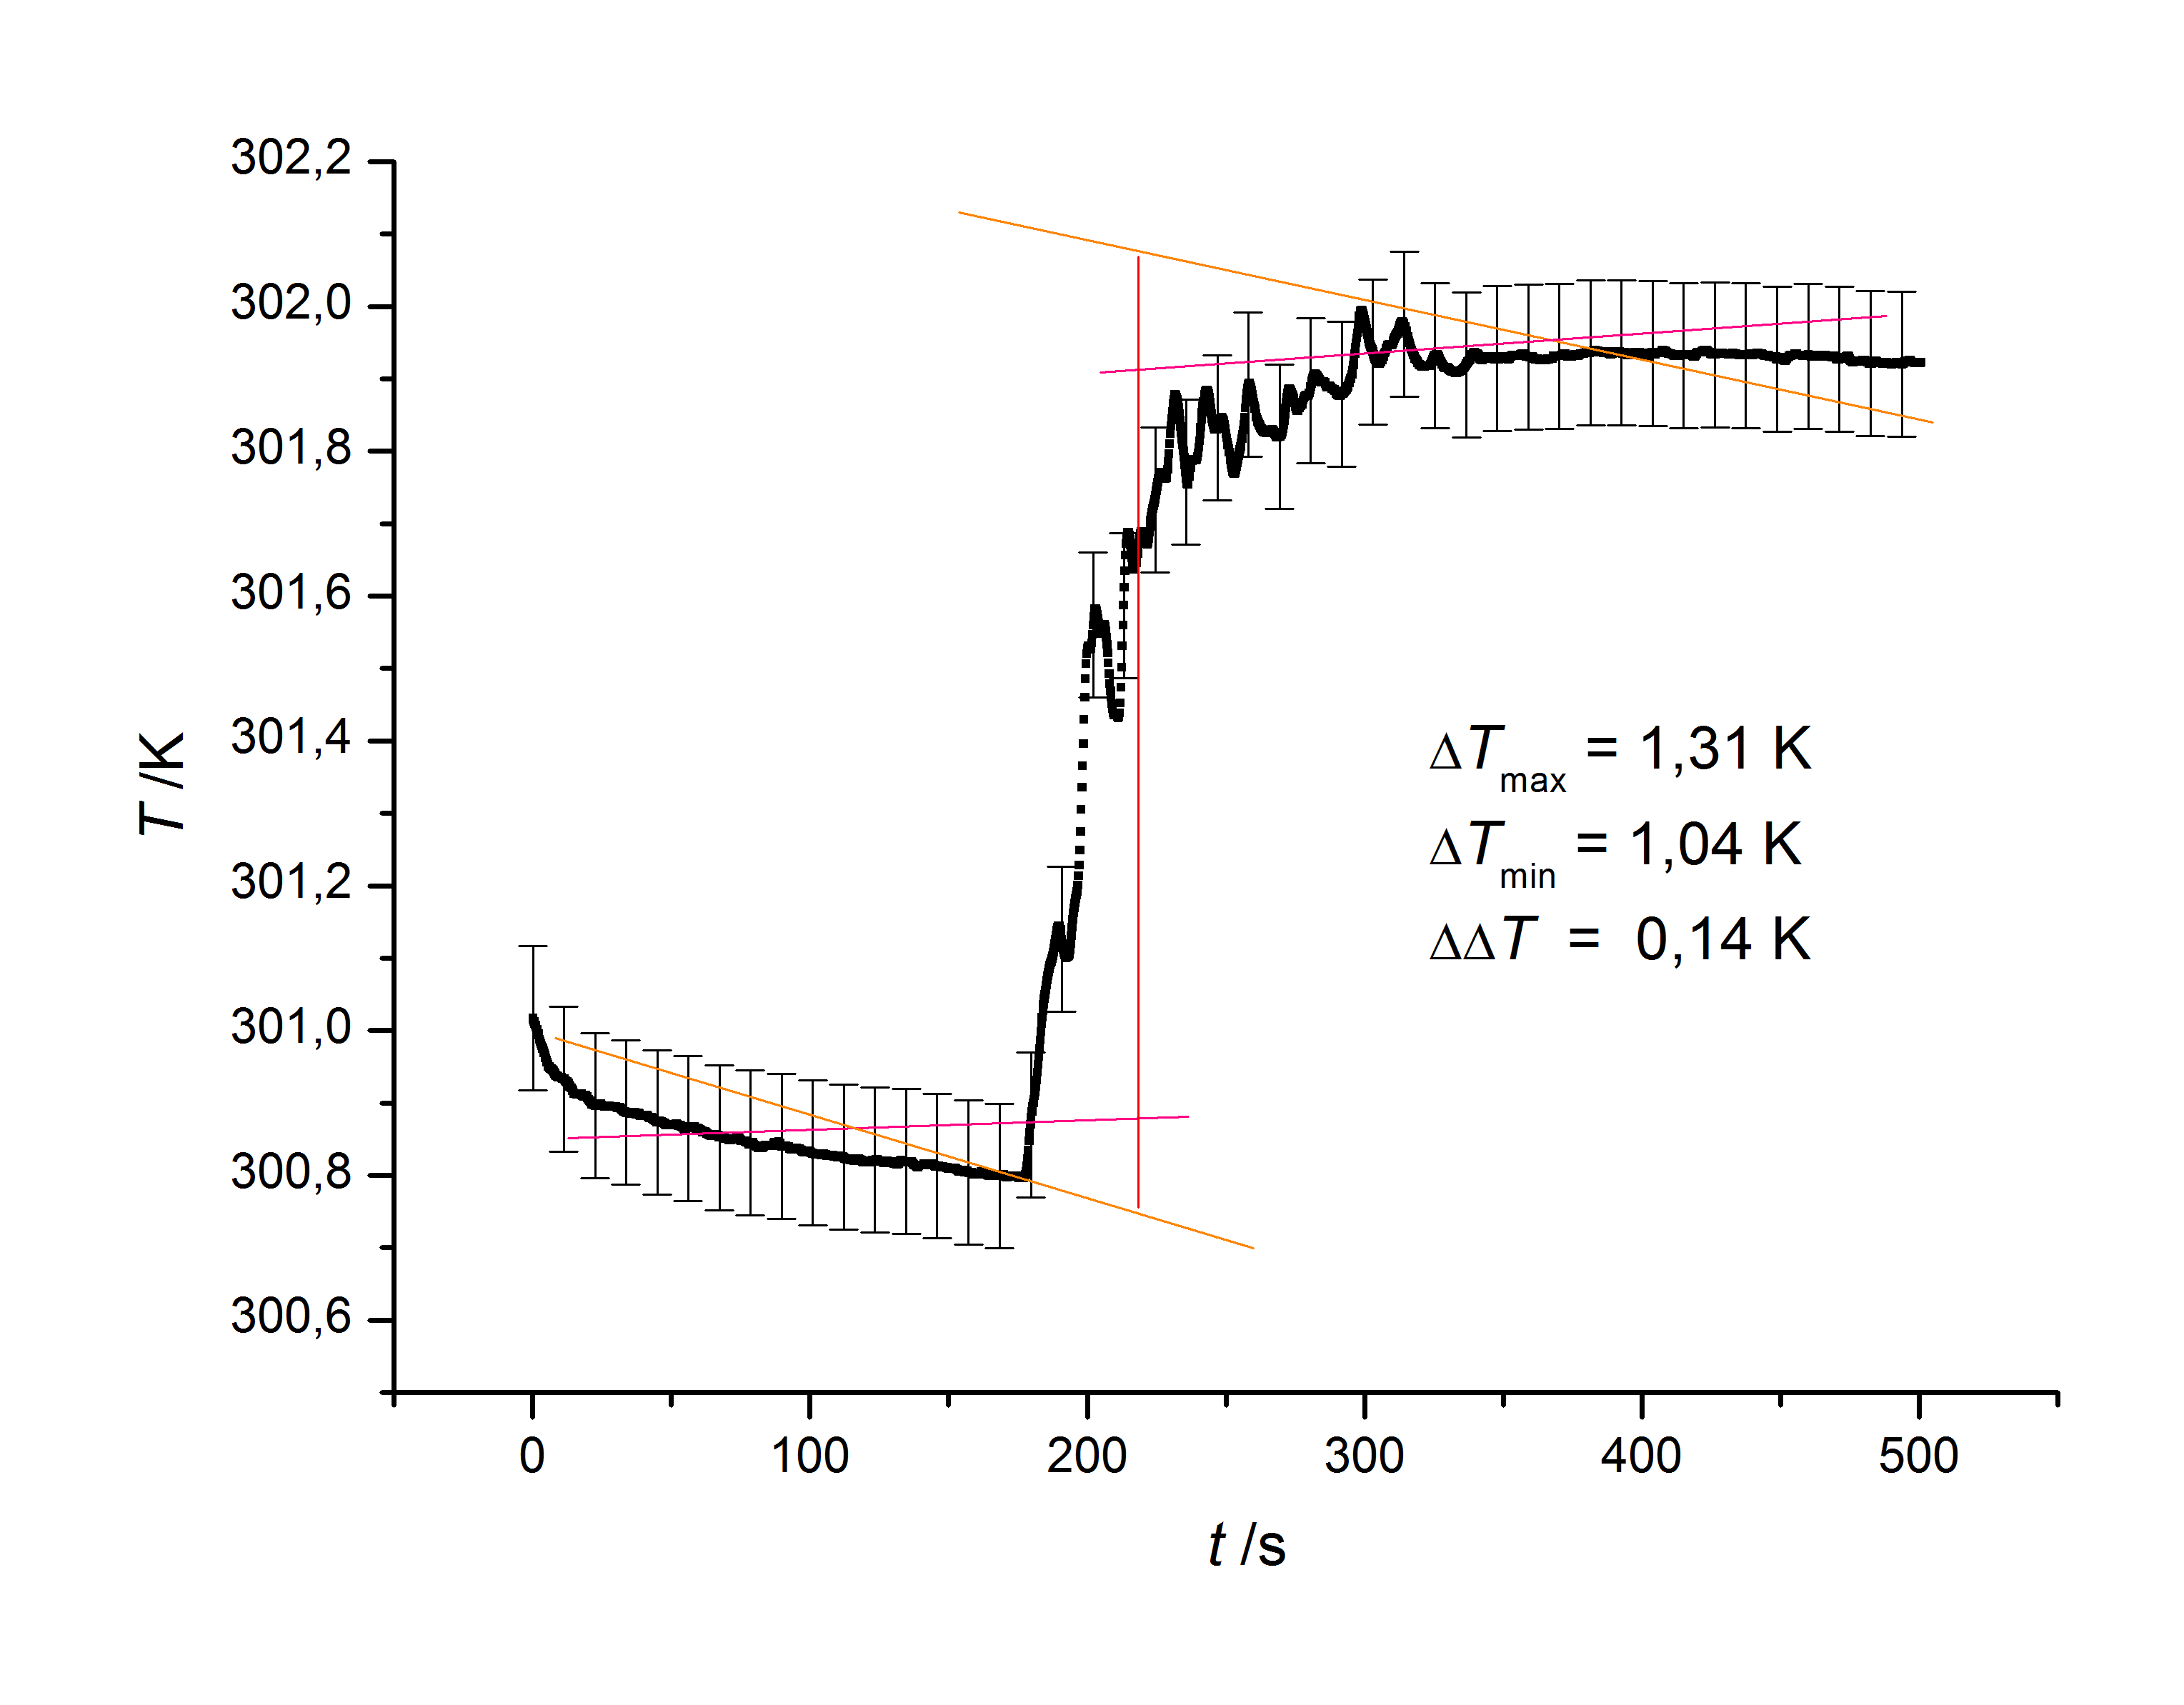
\includegraphics[scale=0.45]{Benz3Fehler.png} \end{center}
\caption{Benzoesäure Messung 3 mit Grenzgeraden.}
\end{figure}

\begin{figure} [h!]
\begin{center}
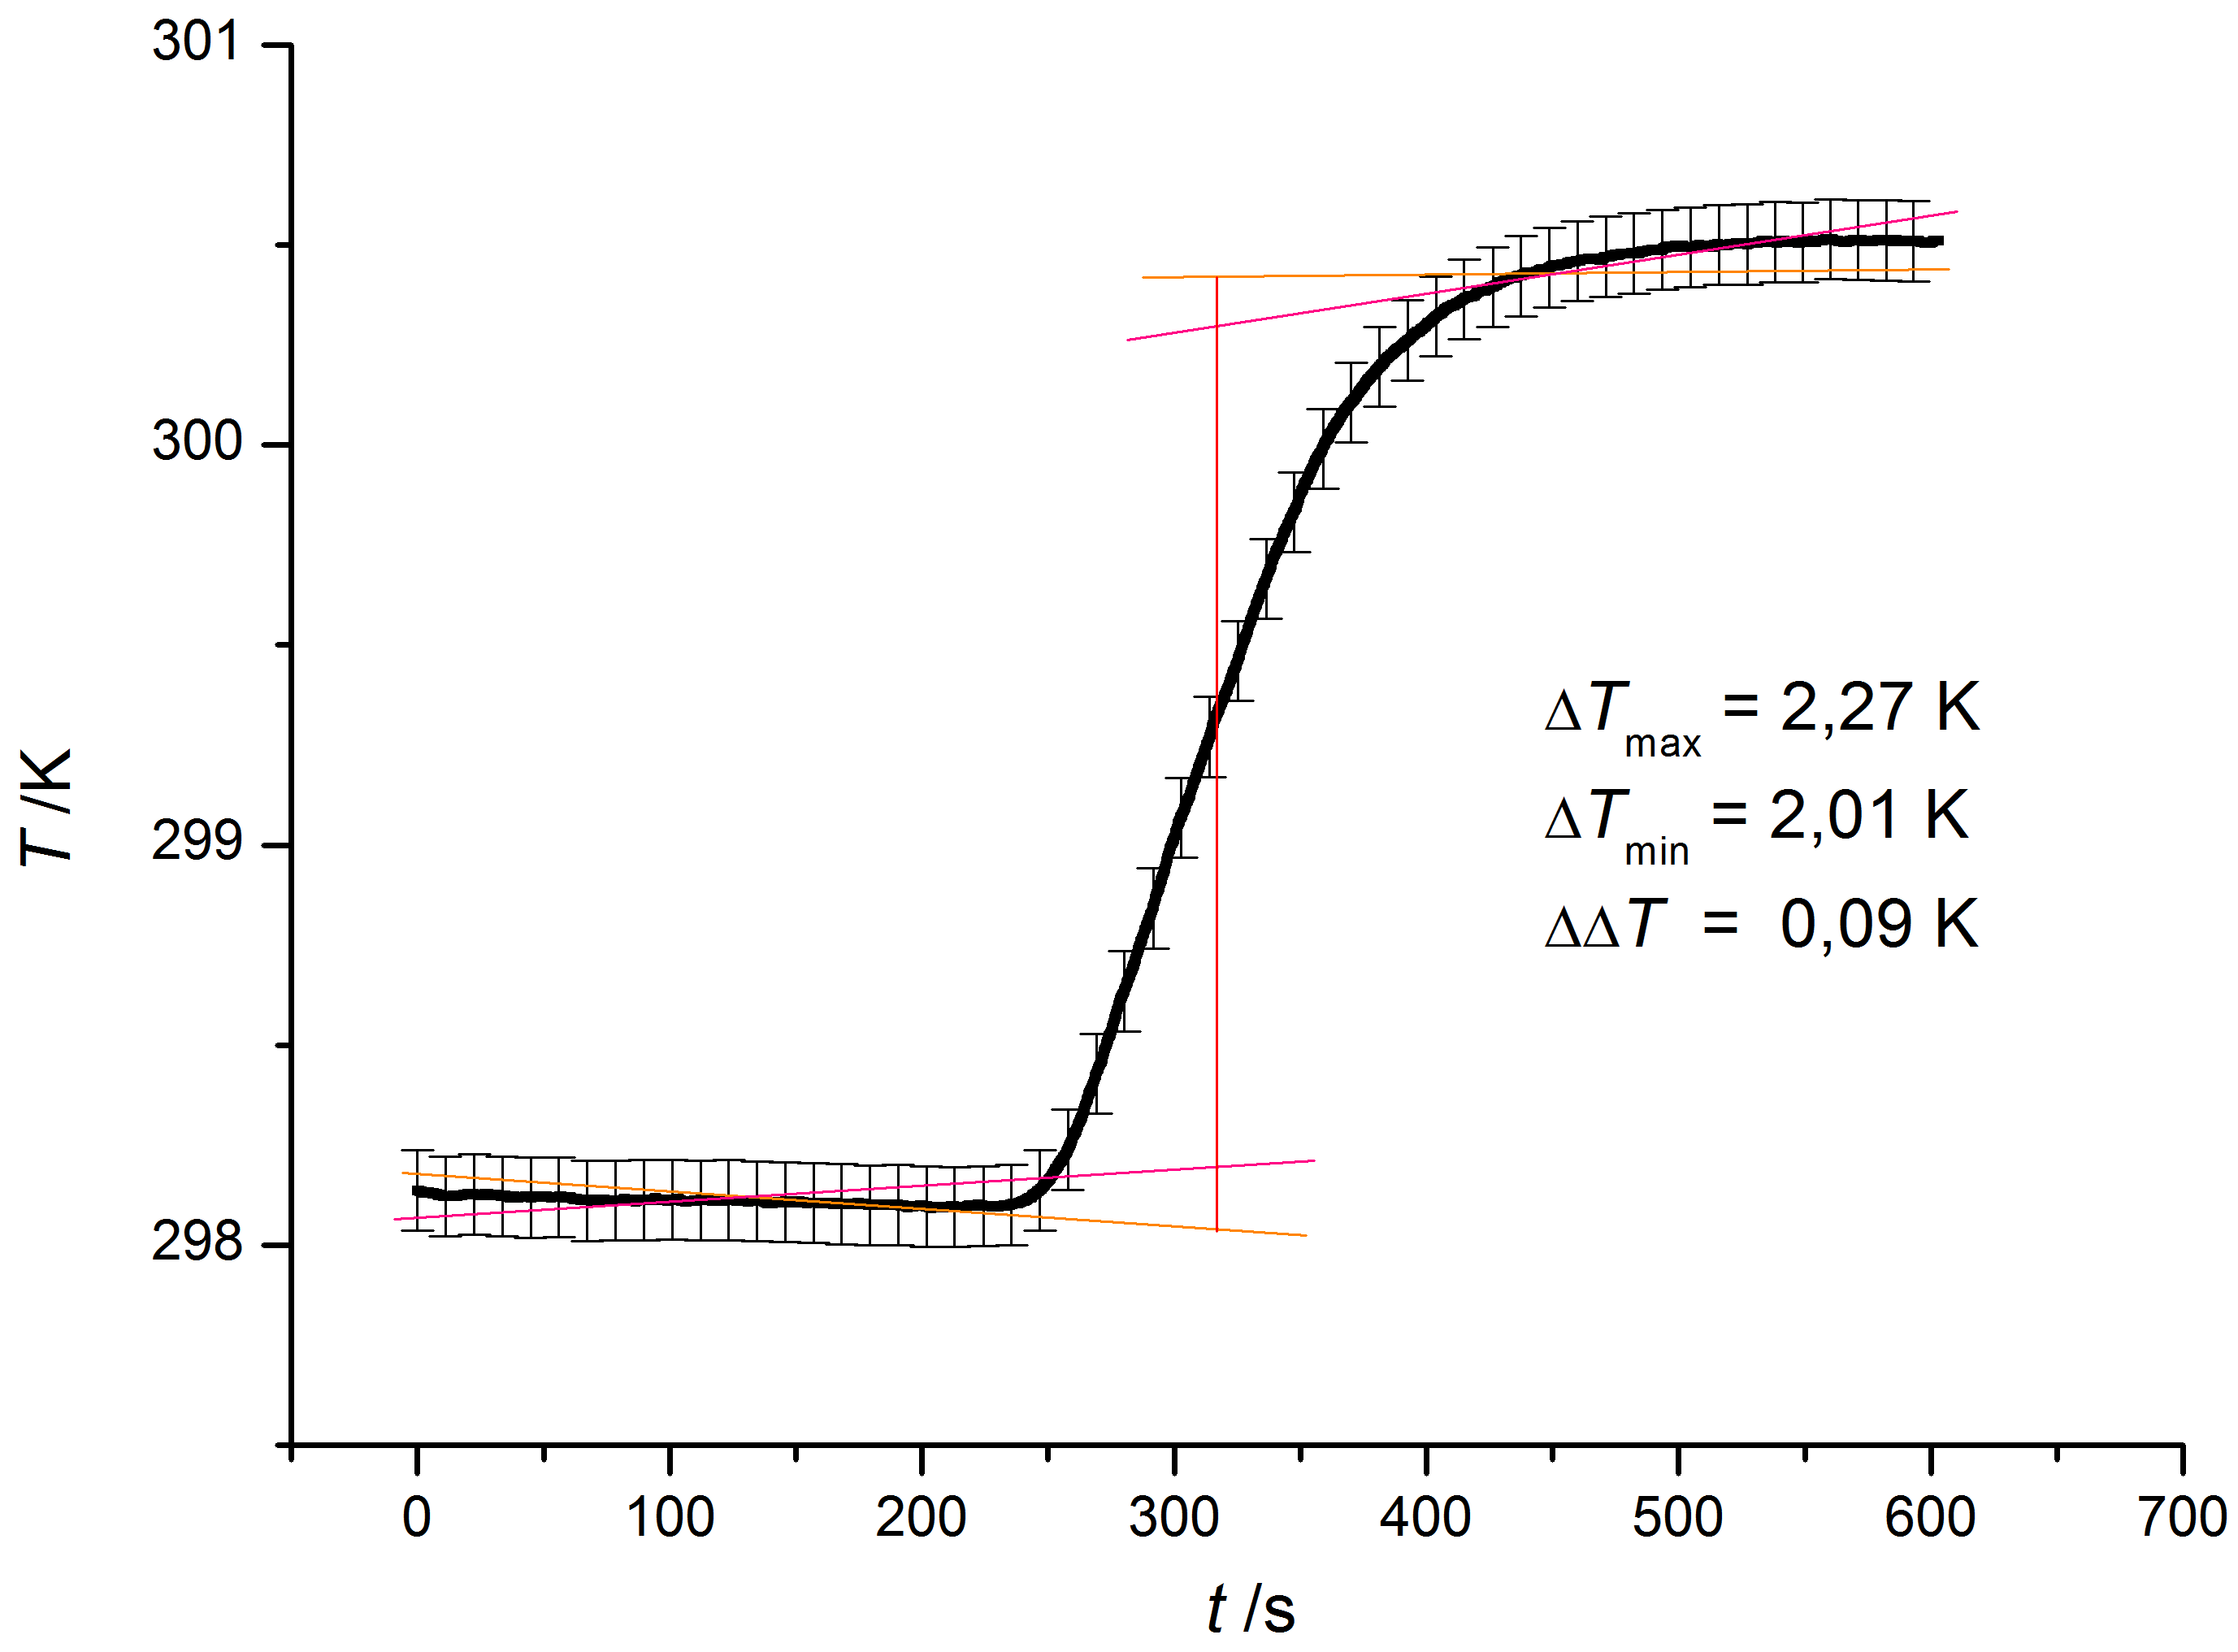
\includegraphics[scale=0.45]{Napht1Fehler.png} \end{center}
\caption{Naphthalin Messung 1 mit Grenzgeraden.}
\end{figure}

\begin{figure} [h!]
\begin{center}
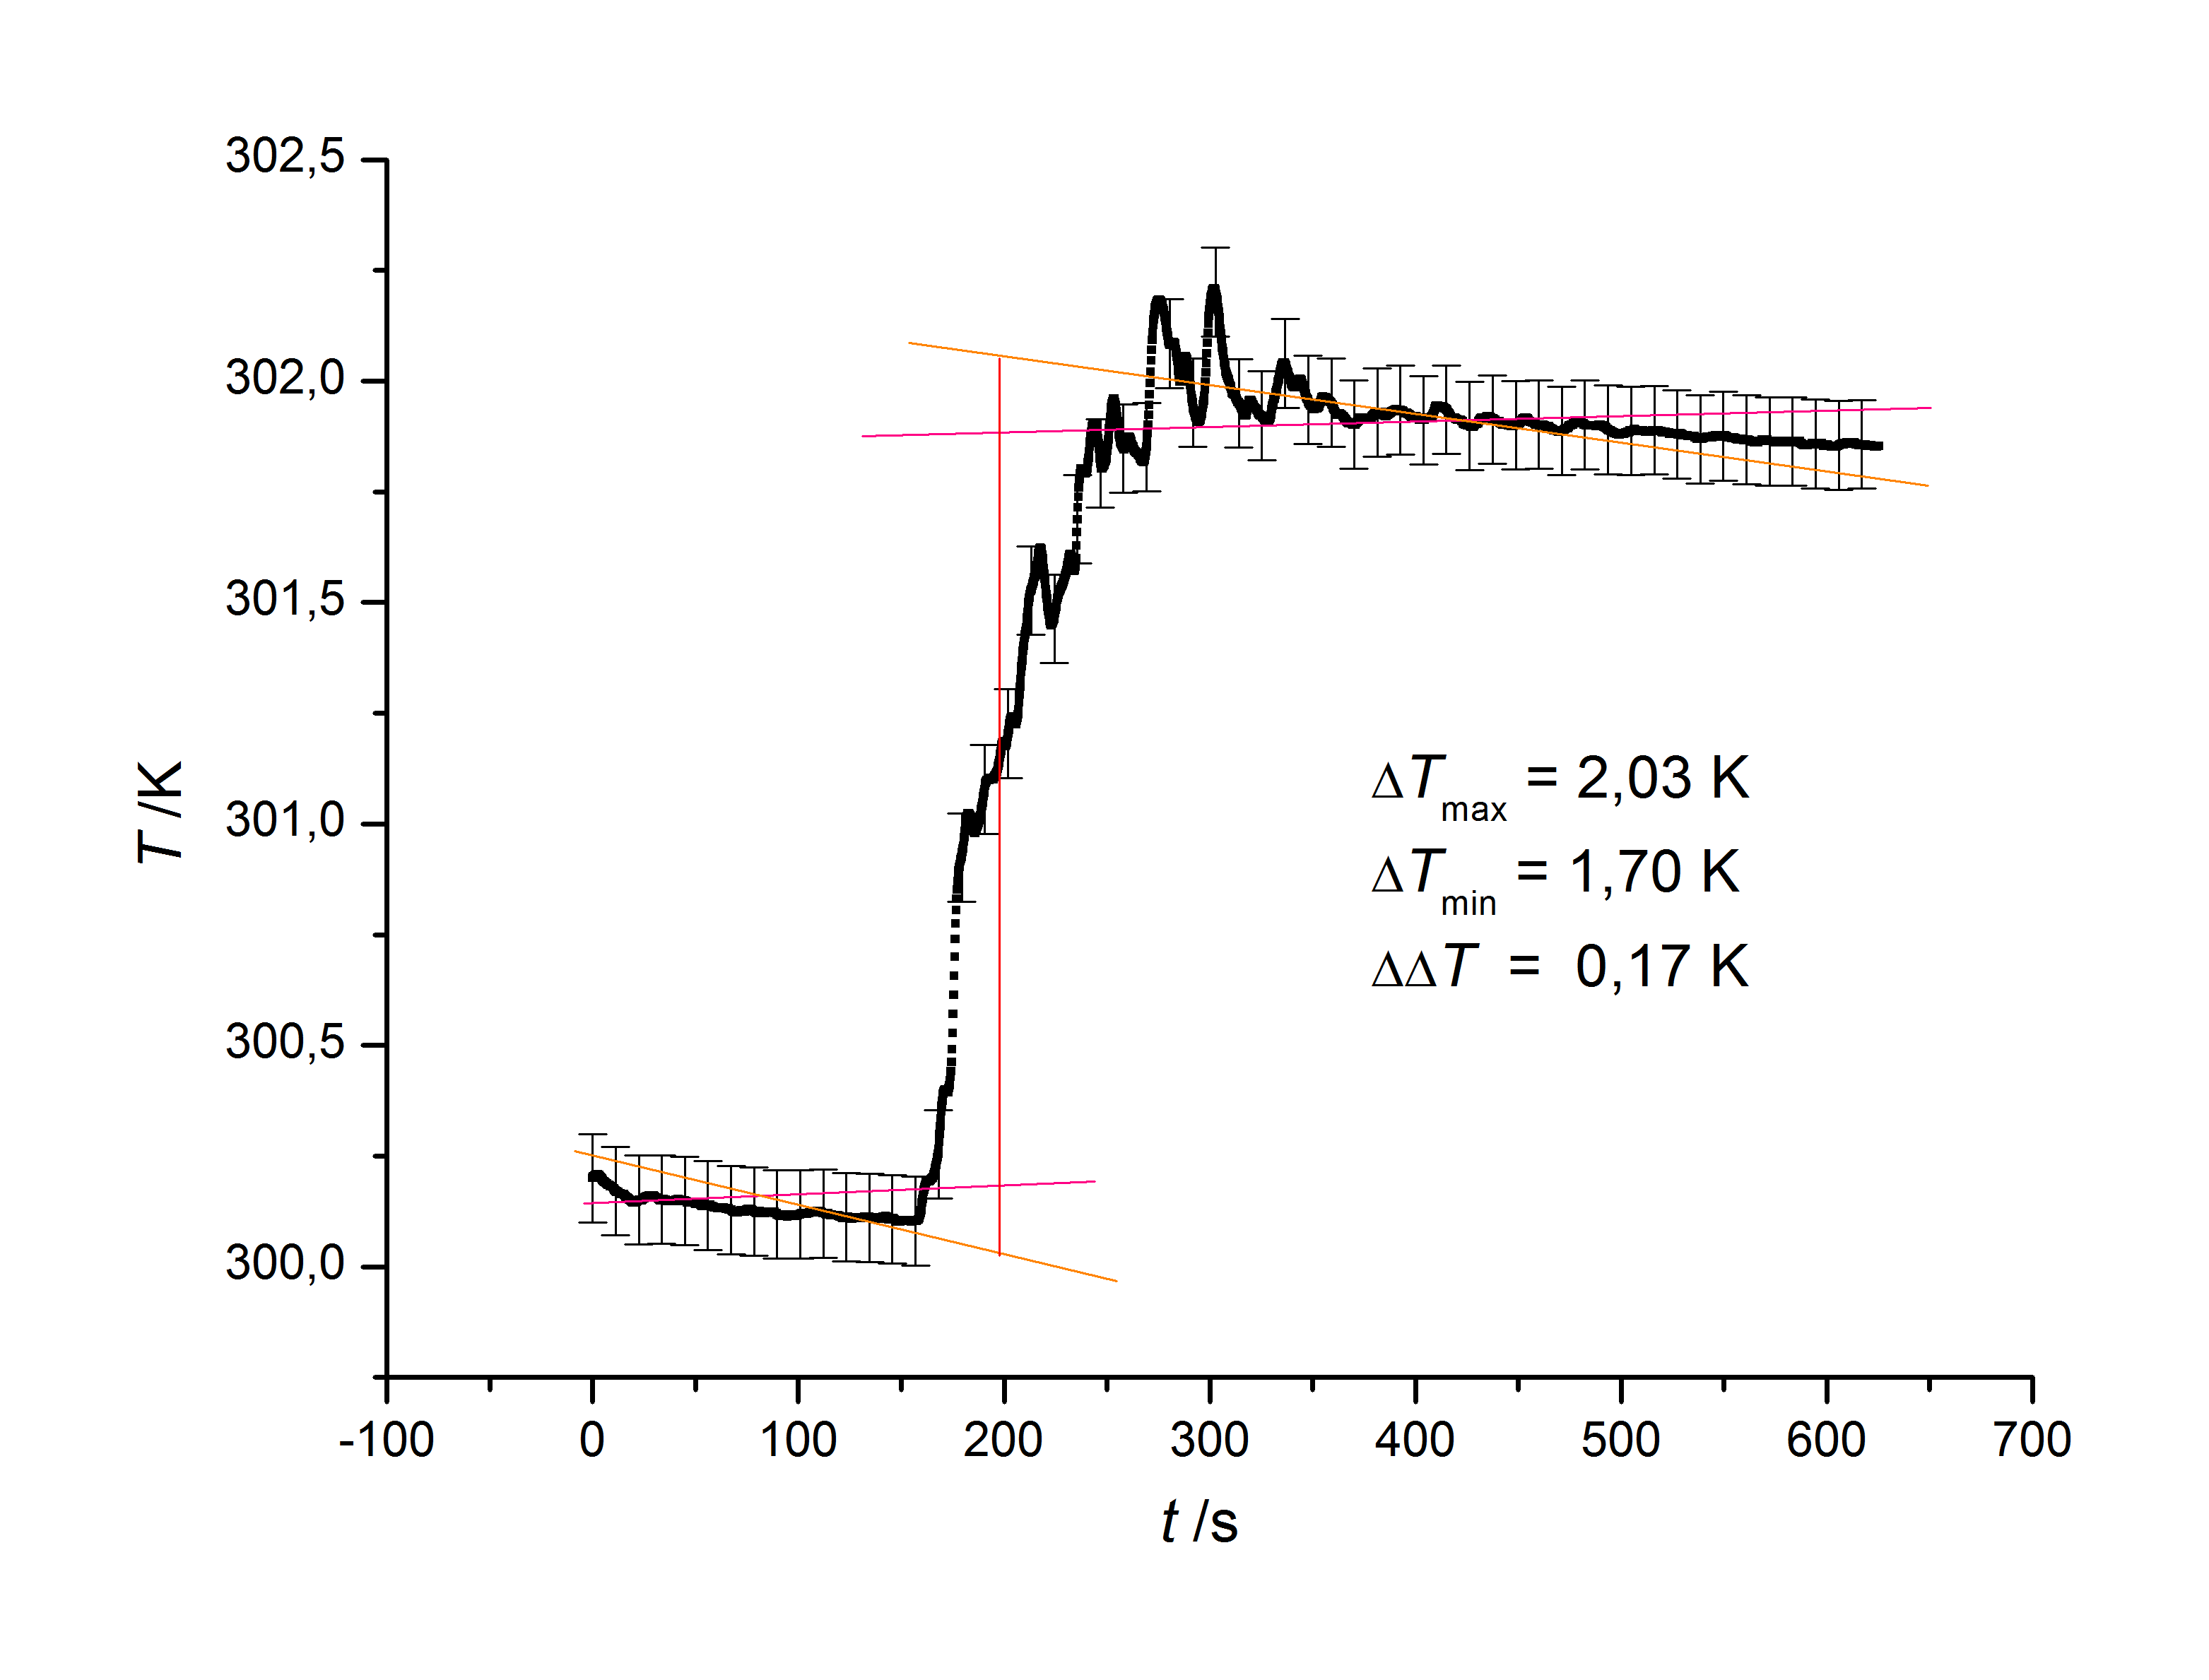
\includegraphics[scale=0.45]{Napht2Fehler.png} \end{center}
\caption{Naphthalin Messung 2 mit Grenzgeraden.}
\end{figure}

\begin{figure} [h!]
\begin{center}
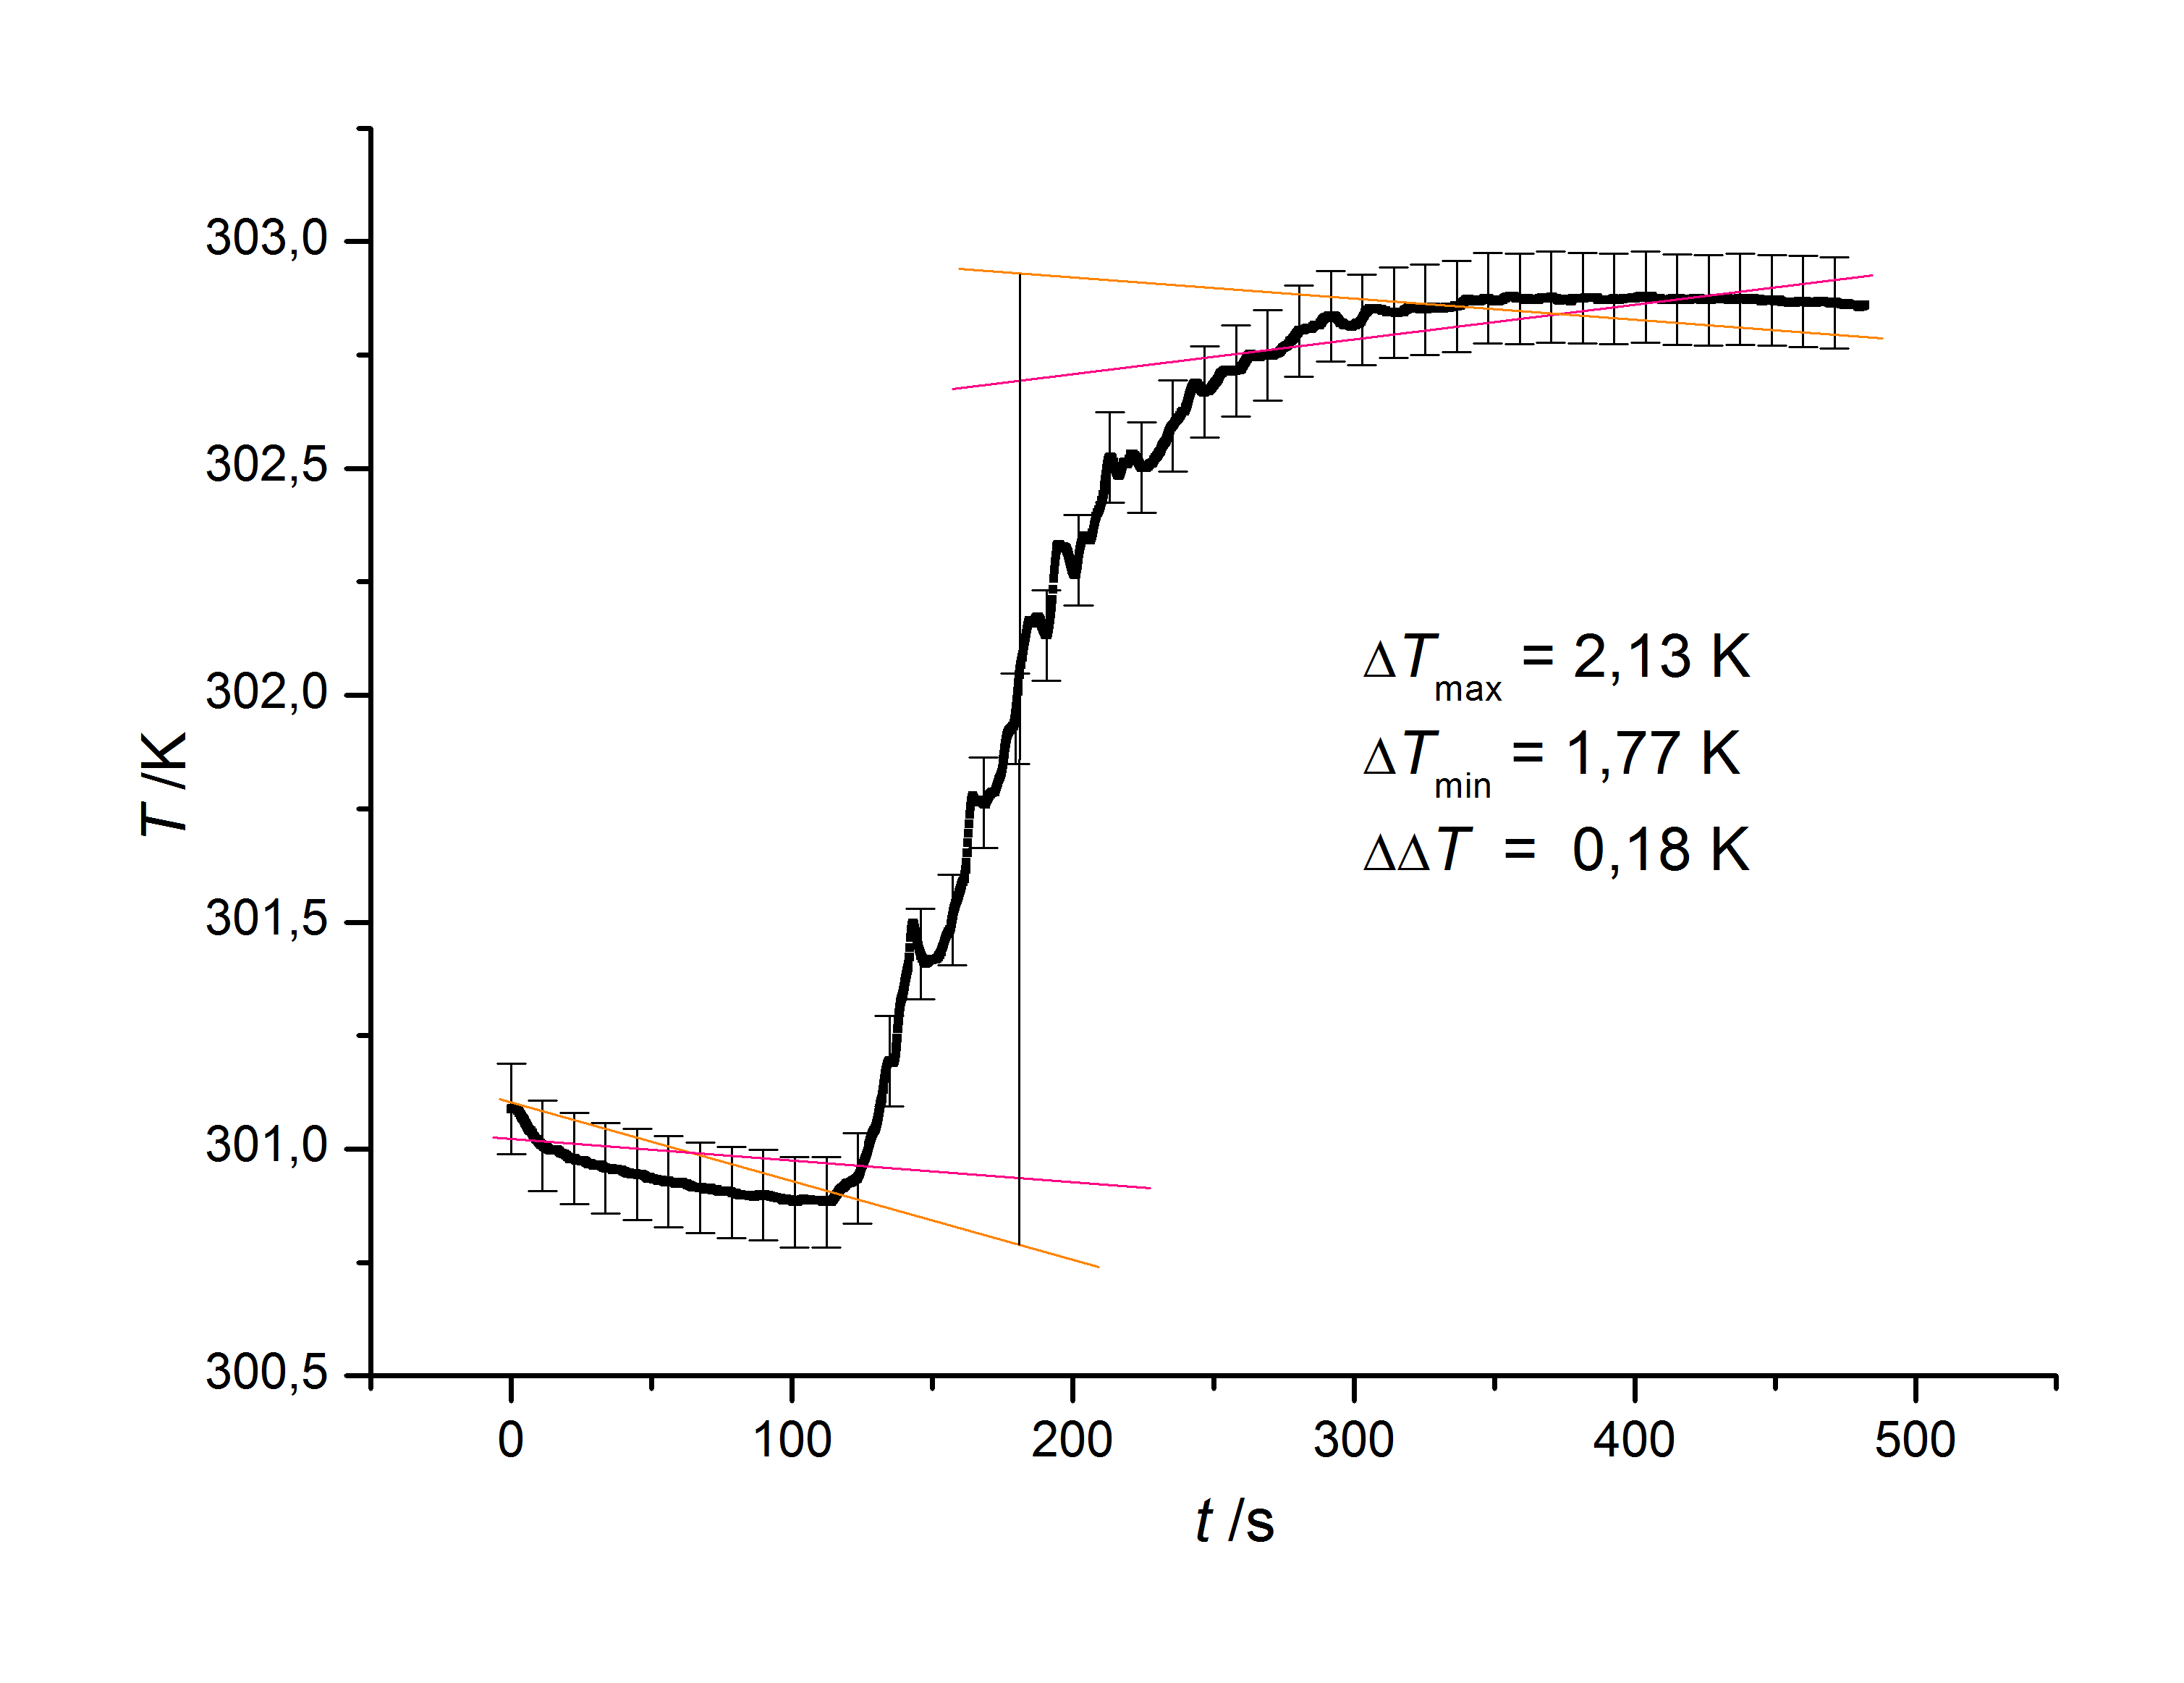
\includegraphics[scale=0.45]{Napht3Fehler.png} \end{center}
\caption{Naphthalin Messung 3 mit Grenzgeraden.}
\end{figure}

\FloatBarrier
\section{Literaturverzeichnis}

1\quad \emph{CRC Handbook of Chemistry and Physics}, 84. Auflage; D.R. Lide; CRC Press LLC: Boca Raton, \textbf{2004}.
\vspace{0,5 cm}


2 \quad \url{http://webbook.nist.gov/cgi/cbook.cgi?ID=C65850&Mask=2}; aufgerufen am 10.12.2016.\\
\vspace{0,5 cm}

3 \quad Atkins, P.W.: \emph{Physikalische Chemie}, Wiley-VCH, Weinheim, \textbf{2006}.\\

%2\quad Kabo, G.J.; Kozyro,A., A.; Frenkel, M.; Blokhin, A. V.\emph{Mol. Cryst. Liq. Cryst.}, \textbf{1999}, \emph{326}, 333-335.

%5\quad Eckhold, Götz: \emph{Praktikum I zur Physikalischen Chemie}, Institut für Physikalische Chemie, Uni Göttingen, \textbf{2014}.

%\vspace{0,5 cm}

%6 \quad Eckhold, Götz: \emph{Statistische Thermodynamik}, Institut für Physikalische Chemie, Uni Göttingen, \textbf{2012}.

%\vspace{0,5cm}

%7 \quad Eckhold, Götz: \emph{Chemisches Gleichgewicht}, Institut für Physikalische Chemie, Uni Göttingen, \textbf{2015}.\\

%\vspace{0,5cm}



%\vspace{0,5cm}

%9 \quad Zemansky: \emph{Heat and Thermodynamics},Mc Graw-Hill, New York, \textbf{1990}.\\

\end{document}
